\documentclass[11pt]{article}

\usepackage{fontspec}
\defaultfontfeatures{Mapping=}    % fontspec's default tex-text mapping
                                   % spuriously emits U+0001 on some inputs
                                   % here; pandoc already writes real Unicode
                                   % dashes/quotes, so this mapping is unneeded
\usepackage{amsmath}
\usepackage{amssymb}
\usepackage{newunicodechar}
% Stray Unicode math symbols appear in plain prose (mostly in the flagged
% "REVISED DRAFT" section, which was typed by hand rather than via Word's
% equation editor) -- map them to their LaTeX math equivalents so they
% render instead of showing as missing-glyph boxes.
\newunicodechar{≥}{\ensuremath{\geq}}
\newunicodechar{≤}{\ensuremath{\leq}}
\newunicodechar{≈}{\ensuremath{\approx}}
\newunicodechar{≠}{\ensuremath{\neq}}
\newunicodechar{∈}{\ensuremath{\in}}
\newunicodechar{→}{\ensuremath{\rightarrow}}
\newunicodechar{±}{\ensuremath{\pm}}
\newunicodechar{×}{\ensuremath{\times}}
\newunicodechar{∑}{\ensuremath{\sum}}
\newunicodechar{√}{\ensuremath{\sqrt{}}}
\newunicodechar{′}{\ensuremath{{}'}}
\newunicodechar{⁻}{\ensuremath{{}^-}}
\newunicodechar{⁴}{\ensuremath{{}^4}}
\newunicodechar{α}{\ensuremath{\alpha}}
\newunicodechar{β}{\ensuremath{\beta}}
\newunicodechar{γ}{\ensuremath{\gamma}}
\newunicodechar{λ}{\ensuremath{\lambda}}
\newunicodechar{μ}{\ensuremath{\mu}}
\newunicodechar{π}{\ensuremath{\pi}}
\newunicodechar{ρ}{\ensuremath{\rho}}
\newunicodechar{τ}{\ensuremath{\tau}}
\newunicodechar{𝒜}{\ensuremath{\mathcal{A}}}
\newunicodechar{𝒮}{\ensuremath{\mathcal{S}}}
\usepackage{graphicx}
\usepackage{longtable}
\usepackage{booktabs}
\usepackage{array}
\usepackage{multirow}
\usepackage{calc}
\newcounter{none}          % pandoc's longtable output sets \LTcaptype{none}
                            % to skip incrementing the table counter when a
                            % caption is baked into the table's own header row
\usepackage{subcaption}
\usepackage{xcolor}                % \colorbox{yellow!40}{...} -- highlights
                                    % carried over from the Word source,
                                    % flagging unresolved citations and other
                                    % author TODOs (soul's \hl breaks under
                                    % XeTeX on Unicode/nested-hyperref text)
\usepackage[margin=1in]{geometry}
\usepackage[style=authoryear,natbib=false,backend=bibtex]{biblatex}
\addbibresource{references.bib}
\usepackage{hyperref}

\title{Integrating Reinforcement Learning and the Theory of Constraints for
Production Scheduling in Stochastic Manufacturing Environments}
\author{}
\date{}

\begin{document}

\maketitle

\begin{abstract}
Modern manufacturing systems often struggle to align demand with capacity,
making production scheduling a critical yet challenging task --- especially
under stochastic conditions. Traditional heuristic and metaheuristic methods
frequently yield suboptimal results due to their limited adaptability.
Reinforcement Learning (RL), known for its ability to make sequential
decisions in uncertain environments, has shown promise in overcoming these
limitations and has outperformed conventional methods in various scheduling
problems. While RL has been integrated with operations management theories
such as Lean and Factory Physics, its combination with the Theory of
Constraints (TOC) --- which focuses on managing system constraints under
variability --- remains underexplored. This study investigates how
integrating RL with TOC can enhance scheduling performance in stochastic
manufacturing environments. We conducted two simulation experiments: one
using a traditional TOC-based scheduling approach, and another combining RL
with TOC. Results show that the RL-TOC hybrid solution achieved superior
performance in terms of both production volume and inventory levels. This
advantage is attributed to the RL agent's ability to adapt to system-wide
work-in-process dynamics, beyond the constraint. We embedded this adaptive
behavior into the traditional TOC scheduling solution, enhancing its
drum-buffer-rope and buffer management components, which we believe is the
main contribution of this study.
\end{abstract}

\noindent\textbf{Keywords:} theory of constraints; reinforcement learning;
production scheduling; production planning and control; manufacturing

\section{Introduction}\label{introduction}

The persistent lack of synchronization between demand and capacity
continues to present significant challenges, even for modern
manufacturing systems (Guo \emph{et al.}, 2024). This mismatch often
arises from the inherent variability within these systems, driven by
factors such as market fluctuations, resource availability, and supply
chain disruptions (Hopp and Spearman, 2021). Effective production
scheduling plays a pivotal role in synchronizing demand with capacity by
defining what to produce, how much to produce, where to produce, and in
what sequence (\colorbox{yellow!40}{cf., Reference ≥ 2021}). Traditionally, production
scheduling has relied on various approaches, ranging from simple
dispatching rules (\colorbox{yellow!40}{e.g., Reference}) to more sophisticated
algorithms (\colorbox{yellow!40}{e.g., Reference ≥ 2021}). Recent advances in the field
have increasingly incorporated meta-heuristics to achieve optimal or
near-optimal solutions (\colorbox{yellow!40}{Reference ≥ 2021}). However, using
meta-heuristics in production scheduling presents challenges,
particularly in dealing with the uncertainty and dynamic conditions
typical of manufacturing environments (\colorbox{yellow!40}{Reference}). Meta-heuristics
such as genetic algorithms, simulated annealing, or tabu search are
often designed for deterministic problems, where environmental
conditions and decision outcomes are fixed (\colorbox{yellow!40}{cf. Reference}). In
contrast, stochastic optimization involves uncertainty and probabilistic
outcomes, which meta-heuristics may struggle to accommodate, often
leading to suboptimal solutions or long computation times
(\colorbox{yellow!40}{Reference}). These algorithms typically rely on heuristics that are
not well-suited to random or fluctuating environments, especially when
applied to large-scale or complex scheduling problems (Márquez and
Ribeiro, 2022). Additionally, meta-heuristics may fail to fully
capitalize on the stochastic nature of the problem, lacking the ability
to learn from past experiences or adjust strategies based on observed
randomness (\colorbox{yellow!40}{Reference}). As a result, this can lead to inefficient
exploration of the solution space and a higher likelihood of converging
to a local optimum rather than a global one (\colorbox{yellow!40}{Reference}).
Furthermore, meta-heuristic algorithms are typically tailored to
specific problems, making them less versatile and prone to poor
generalization (\colorbox{yellow!40}{Reference}). To overcome these challenges,
reinforcement learning (RL) has emerged as a promising alternative for
production scheduling (\colorbox{yellow!40}{Reference ≥ 2021}). RL is a branch of machine
learning where an agent interacts with its environment to maximize
long-term rewards (Sutton and Barto, 2018). Its capacity to make
sequential decisions and adapt to stochastic environments makes RL
especially suitable for production scheduling applications (\colorbox{yellow!40}{cf., Li
et al., 2022; del Real Torres et al., 2022; Wang et al., 2022}).

RL has proven effective in various manufacturing contexts. For instance,
Tang and Salonitis (\colorbox{yellow!40}{2021}) leveraged deep RL with discrete-event
simulation to optimize scheduling in reconfigurable systems, surpassing
conventional dispatching rules. Chen et al. (\colorbox{yellow!40}{2022}) addressed the
flexible job shop scheduling problem with resource preemption using a
deep RL-based algorithm, outperforming traditional meta-heuristics. Liu
et al. (\colorbox{yellow!40}{2022}) applied a Deep Q-Network algorithm for real-time
scheduling in dynamic flexible job shop manufacturing. Gerpott et al.
(\colorbox{yellow!40}{2022}) used the Actor-Critic algorithm to minimize tardiness and
makespan in a two-stage hybrid flow shop. Beyond standalone
applications, RL has been integrated with some operations management
(OM) theories. For example, Silva and Azevedo (\colorbox{yellow!40}{2019}) applied RL to
optimize work-in-process (WIP) caps in CONWIP and push systems,
achieving a substantial reduction in WIP without sacrificing production
volume. Xanthopoulos et al. (\colorbox{yellow!40}{2019}) demonstrated RL's superiority in
deriving optimal control policies for CONWIP-type systems. Paraschos et
al. (\colorbox{yellow!40}{2023}) used RL to optimize a three-stage production line,
promoting Lean practices. Lahrichi et al. (\colorbox{yellow!40}{2023}) used SARSA
algorithm to dynamically parameterize demand-driven material
requirements planning, reducing inventory and preventing stockouts.

One OM theory that has yet to be explored with RL in production
scheduling is the Theory of Constraints (TOC). Like RL, which addresses
decision-making in stochastic environments, TOC also does so, but with a
strict focus on the constraint that limits the system's overall
performance, usually protecting it through the use of buffers (Goldratt
and Cox, 1984a). In production scheduling, TOC introduces two prominent
techniques (Goldratt, 2006a; Schragenheim and Ronen, 1990): (i)
drum-buffer-rope (DBR); and (ii) buffer management (BM). When applied
together, these techniques, along with their associated performance
measures --- throughput, inventory, and operating expenses --- enable
the effective management of highly interdependent systems
(\colorbox{yellow!40}{Reference}). They achieve this by protecting capacity-constrained
resources against shortages or blockages through inventory buffers while
synchronizing inflows to the rhythm of the constraint (\colorbox{yellow!40}{Reference}).
TOC-based solutions to scheduling problems have demonstrated their
effectiveness in various contexts. For instance, they have improved
efficiency in production lines within aerospace engineering-to-order
facilities (Telles \emph{et al.}, 2022a) and increased productivity in
small and medium-sized manufacturing enterprises (Buestán Benavides and
Van Landeghem, 2015). Furthermore, these solutions have been
successfully applied to automotive parts manufacturing (Golmohammadi,
2015), LCD panel production (Wu \emph{et al.}, 2010), and engine
cylinder restoration (Ma and Chen, 2009).

Despite the promising synergy between RL and TOC in production
scheduling, their integration remains largely unexplored. This gap
prompts the following research questions: (i) how can RL and TOC be
combined to address production scheduling in stochastic manufacturing
environments? (ii) what practical and theoretical outcomes can result
from this combination? To address these questions, we employed
computational simulation and conducted two experiments within the same
stochastic manufacturing environment. In the first experiment,
production scheduling was performed using a TOC-based solution (i.e.,
DBR and BM). In the second, scheduling was carried out combining RL with
TOC. From a pragmatic perspective, a summative evaluation comparing
these experiments demonstrated that a scheduling solution combining RL
and TOC outperformed the TOC-based solution in terms of both production
volume and inventory levels. Theoretically, a formative evaluation
revealed that this advantage stems from the RL agent's ability to
monitor and adapt to system-wide WIP dynamics, rather than focusing
solely on the constraint. We embedded this adaptive behavior into the
traditional TOC scheduling solution, enhancing its DBR and BM
components, which we believe is the main contribution of this study.

The remainder of this paper is structured as follows. Section 2 provides
the theoretical background on both RL and the TOC in the context of
production scheduling. Section 3 outlines the research design, while
Section 4 details the development of simulation models. Section 5
describes the setup of the simulation experiments, with the
corresponding summative and formative evaluations presented in Section
6. Finally, Section 7 discusses the results, and Section 8
contextualizes the research contributions and limitations, highlighting
opportunities for future studies.

\section{Theoretical Background}\label{theoretical-background}

\subsection{Reinforcement Learning}\label{reinforcement-learning}

RL is a branch of machine learning characterized by two core components
(\colorbox{yellow!40}{Reference}): (i) the agent; and (ii) the environment. The agent
observes the current state of the environment, selects an action, and
receives feedback in the form of a reward associated with that action
(Sutton and Barto, 2018). Through iterative interactions with the
environment, the agent refines its decision-making strategy, or policy,
to maximize long-term rewards (Esteso \emph{et al.}, 2023). Unlike
traditional machine learning approaches that rely on static,
pre-existing datasets, RL agents learn from dynamic, continuously
evolving datasets generated through their ongoing interaction with a
virtual environment (Panzer and Bender, 2022). This environment is often
modeled using discrete-event simulation, which effectively captures
system dynamics and variability (Kuhnle \emph{et al.}, 2022; Nguyen
\emph{et al.}, 2022).

RL problems are typically framed as a sequence of interactions between
the agent and the environment at discrete time steps
\(t \in \left\{ 0,\ 1,\ 2,\ \ldots,T \right\}\) (\colorbox{yellow!40}{Reference}). At
each time step \(t\), the agent receives a representation of the
environment's state, \(S_{t}\mathcal{\in S}\), where \(\mathcal{S}\) is
the set of possible states (\colorbox{yellow!40}{Reference}). Based on this state, the
agent selects an action, \(A_{t}\mathcal{\in A(}S_{t})\), where
\(\mathcal{A(}S_{t})\) represents the set of actions available in state
\(S_{t}\) (\colorbox{yellow!40}{Reference}). One time step later, as a result of its
action, the agent receives a numerical reward,
\(R_{t + 1}\mathcal{\in R \subset}\mathbb{R}\), and transitions to a new
state, \(S_{t + 1}\) (\colorbox{yellow!40}{Reference}). In manufacturing applications of
RL, the environment corresponds to the manufacturing system itself (or a
model of it), such as an assembly line or warehouse (\colorbox{yellow!40}{e.g.,
Reference}). The agent acts as the decision-maker, which could be a
production scheduler, for example (\colorbox{yellow!40}{e.g., Reference}). The state
represents the current status of the system, such as the number of
machines that are idle, running, or under maintenance (\colorbox{yellow!40}{e.g.,
Reference}). The action refers to a decision the agent makes within the
system, such as assigning a new work order to a machine or adjusting the
priority of a pending job (\colorbox{yellow!40}{e.g., Reference}). The reward represents
the payoff the agent receives in response to its actions, typically
aimed at improving a specific performance measure, such as production
volume or lead time (\colorbox{yellow!40}{e.g., Reference}).

The environment in RL can be deterministic or stochastic. In the latter
case, it is often modeled as a finite Markov Decision Process (MDP),
where the environment's response at \(t + 1\) depends only on the state
and action representations at \(t\) (\colorbox{yellow!40}{Reference}). This assumption
simplifies the dynamics of agent-environment interactions, which can be
described by a distribution function, such as (\colorbox{yellow!40}{Reference}):

\begin{equation}
p\left( s',r \middle| s,a \right) = \Pr\left\{ S_{t + 1} = s',\ R_{t + 1} = r \middle| S_{t} = s,A_{t} = a \right\}
\tag{1}
\end{equation}

for all possible states \(s\), \(s'\), rewards \(r\), and actions \(a\).
This formulation allows prediction of the next state and expected reward
based on the current state and action, though it requires prior
knowledge on the distribution function (\colorbox{yellow!40}{Reference}).

The agent's behavior is governed by a policy,
\(\pi_{t}\left( a \middle| s \right)\), which represents the probability
of taking action \(A_{t} = a\) in state \(S_{t} = s\) (\colorbox{yellow!40}{Reference}).
If the policy involves no randomness, then only one action can be taken
from each state, resulting in a deterministic policy \(\pi_{t}(s)\)
(\colorbox{yellow!40}{Reference}). RL methods define how the agent updates its policy
based on its experiences, with the ultimate goal of maximizing the total
rewards received over time, known as the return \(G_{t}\):

\begin{equation}
G_{t} = \sum_{k = 0}^{T - t - 1}{\gamma^{k}R_{t + k + 1},}
\tag{2}
\end{equation}

where \(\gamma\) is the discount rate \((0 \leq \gamma \leq 1)\) that
determines the present value of future rewards (\colorbox{yellow!40}{Reference}). A
reward received \(k\) time steps in the future is worth only
\(\gamma^{k - 1}\) times its immediate value.

Most RL algorithms rely on estimating value functions, which assess the
`goodness' of being in a given state or taking a specific action
(\colorbox{yellow!40}{Reference}). This goodness is defined in terms of the expected
return \(\mathbb{E}_{\pi}\lbrack.\rbrack\) and is essential for
identifying optimal policies \(\pi_{*}\), where
\(\upsilon_{*}(s) \geq \upsilon_{\pi}(s)\) or
\(q_{*}(s,a) \geq q_{\pi}(s,a)\) for all \(s \in \mathcal{S}\) and
\(a \in \mathcal{A}\), (\colorbox{yellow!40}{cf., Reference}). The two primary value
functions for finite MDPs are (\colorbox{yellow!40}{Reference}):

\begin{enumerate}
\def\labelenumi{\roman{enumi}.}
\item
  State-value function \((\upsilon_{\pi}(s))\): The expected return
  starting in state \(s\) and following policy \(\pi\):
\end{enumerate}

\begin{equation}
\upsilon_{\pi}(s) = \mathbb{E}_{\pi}\left\lbrack G_{t}|S_{t} = s \right\rbrack = \mathbb{E}_{\pi}\left\lbrack \left. \ \sum_{k = 0}^{T - t - 1}{\gamma^{k}R_{t + k + 1}} \right|S_{t} = s \right\rbrack;
\tag{3}
\end{equation}

\begin{enumerate}
\def\labelenumi{\roman{enumi}.}
\setcounter{enumi}{1}
\item
  Action-value function \((q_{\pi}(s,a))\): The expected return starting
  from state \(s\), taking action \(a\), and subsequently following
  policy \(\pi\):
\end{enumerate}

\begin{equation}
q_{\pi}(s,a) = \mathbb{E}_{\pi}\left\lbrack G_{t}|S_{t} = s,A_{t} = a\  \right\rbrack = \mathbb{E}_{\pi}\left\lbrack \left. \ \sum_{k = 0}^{T - t - 1}{\gamma^{k}R_{t + k + 1}} \right|S_{t} = s,\ A_{t} = a \right\rbrack.
\tag{4}
\end{equation}

Value functions satisfy recursive relationships, which allows the use of
Bellman optimality equation (\colorbox{yellow!40}{cf., Reference}). This leads to the
optimal forms of the state-value function \({(\upsilon}_{*}(s))\) and
the action-value function \({(q}_{*}(s,a)\)), defined as follows
(\colorbox{yellow!40}{Reference}):

\begin{equation}
\upsilon_{*}(s) = \max_{a \in A(s)}{\sum_{s',r}^{}{p\left( s',r \middle| s,a \right)\left\lbrack r + \gamma\upsilon_{*}(s') \right\rbrack}.}
\tag{5}
\end{equation}

\begin{equation}
q_{*}(s,a) = \sum_{s',r}^{}{p\left( s',r \middle| s,a \right)}\left\lbrack r + \gamma\max_{a'}{q_{*}(s',a')} \right\rbrack.
\tag{6}
\end{equation}

The computation of optimal policies depends on how the agent predicts
the environment\textquotesingle s response to its actions
(\colorbox{yellow!40}{Reference}). In model-based methods, where the agent uses a model
to plan actions in advance, such as estimating
\(p\left( s',r \middle| s,a \right)\), dynamic programming algorithms
are typically employed (\colorbox{yellow!40}{e.g., Reference}). In contrast, model-free
methods focus on learning the direct relationship between actions and
returns through `trial and error', often utilizing temporal-difference
algorithms (\colorbox{yellow!40}{Reference}). Model-free methods can be further divided
into on-policy and off-policy strategies (\colorbox{yellow!40}{Reference}). An on-policy
strategy learns from the actions taken by the current policy, with SARSA
being the prominent learning algorithm (\colorbox{yellow!40}{e.g., Reference}), while an
off-policy strategy learns from actions taken by a combination of the
current and different policies, typically implemented using the
Q-learning algorithm (\colorbox{yellow!40}{e.g., Reference}). Furthermore, model-free
methods can be categorized into gradient-based and gradient-free
methods. Gradient-based methods, such as Proximal Policy Optimization
(PPO), optimize policies by directly adjusting parameters in the
direction of the gradient of the expected return with respect to the
policy parameters (\colorbox{yellow!40}{Reference}). The PPO algorithm specifically
improves upon traditional policy gradient methods by employing a clipped
objective function to prevent large updates that could destabilize
training (\colorbox{yellow!40}{Reference}). The core PPO objective is expressed as
follows:

\begin{equation}
L^{CLIP}(\theta) = \mathbb{E}_{t}\left\lbrack \min\left( p_{t}(\theta){\widehat{A}}_{t},\ clip(p_{t}(\theta),1 - \epsilon,1 + \epsilon){\widehat{A}}_{t} \right) \right\rbrack;
\tag{7}
\end{equation}

where
\(p_{t}(\theta) = \frac{\pi_{\theta}\left( a|s \right)}{\pi_{\theta_{old}}\left( a|s \right)}\)
is the probability ratio,
\({\widehat{A}}_{t} = G_{t} - \upsilon_{\pi}(s)\) is the estimated
advantage, and \(\epsilon\) is a small hyperparameter controlling the
clipping range. This method ensures that the updates are stable and
avoid excessively large policy changes (\colorbox{yellow!40}{Reference}). Gradient-free
methods, on the other hand, typically rely on search-based techniques or
evolutionary strategies to update the policy without directly computing
gradients (\colorbox{yellow!40}{Reference}). These methods are particularly useful in
environments where the gradient is difficult to compute or highly noisy
(\colorbox{yellow!40}{Reference}). More recently, both model-based and model-free methods
have incorporated deep learning, leading to algorithms like Actor-Critic
and Deep Q-Network (\colorbox{yellow!40}{e.g., Reference 1, Reference 2}), which have
paved the way for a new branch of RL known as deep RL (\colorbox{yellow!40}{cf.,
Reference}). The ability to make autonomous sequential decisions and
adapt to stochastic environments makes RL particularly well-suited for
production scheduling applications (\colorbox{yellow!40}{cf., Reference 1, Reference 2}),
providing a foundation for the remainder of this work.

\subsection{Theory of Constraints}\label{theory-of-constraints}

A constraint is any factor that prevents a system from achieving its
goal (Mabin and Balderstone, 2003). In manufacturing environments,
constraints can take the form of equipment with limited capacity or low
reliability, operations that produce high rates of defective parts, or
policies that limit the system's flexibility or efficiency (Gupta and
Boyd, 2008). Addressing the system's constraint often involves five
major steps (Watson \emph{et al.}, 2007): (i) identify the system's
constraint; (ii) exploit the constraint; (iii) subordinate everything
else to the constraint; (iv) elevate the constraint; and (v) if the
constraint is resolved, restart the process from step (i).

When demand \(d\) exceeds the planned capacity \(p\), identifying the
system's constraint (step 1) requires locating the resource
\(j \in \left\{ 0,\ 1,\ 2,\ \ldots,J \right\}\) with the highest load
\(l_{j}\), defined as \({argmax}_{j}l_{j}\) (\colorbox{yellow!40}{Reference}). In a
stochastic manufacturing environment producing multiple products
\(i \in \left\{ 0,\ 1,\ 2,\ \ldots,I \right\}\) in quantities \(m_{i}\),
utilizing \(J\) resources with expected cycle times
\(\mathbb{E}\left\lbrack \mathcal{T}_{ij}^{c} \right\rbrack\)\hspace{0pt},
considering each resource's expected overall effectiveness
\(\mathbb{E}\left\lbrack \mathcal{E}_{j} \right\rbrack\)\hspace{0pt}\hspace{0pt}
and change-over time
\(\mathbb{E}\left\lbrack \mathcal{T}_{j}^{CT} \right\rbrack\), the load
on a resource can be calculated as follows (\colorbox{yellow!40}{Reference}):

\begin{equation}
d = \left. \ \sum_{\forall i}^{}{m_{i}\max\left( \frac{\mathbb{E}\left\lbrack \mathcal{T}_{ij}^{c} \right\rbrack}{\mathbb{E}\left\lbrack \mathcal{E}_{j} \right\rbrack} + \frac{\mathbb{E}\left\lbrack \mathcal{T}_{j}^{CT} \right\rbrack}{m_{i}} \right)} \right|D_{i} \in D \land D = d;
\tag{8}
\end{equation}

\begin{equation}
\left. \ l_{j} = \frac{1}{p}\left\lbrack \left( \sum_{\forall i}^{}{m_{i}\frac{\mathbb{E}\left\lbrack \mathcal{T}_{ij}^{c} \right\rbrack}{\mathbb{E}\left\lbrack \mathcal{E}_{j} \right\rbrack}} \right)\mathbb{+ E}\left\lbrack \mathcal{T}_{j}^{CT} \right\rbrack \right\rbrack \right|d \geq p.
\tag{9}
\end{equation}

Once the constraint is identified, the next step is to determine the
most effective way to exploit it (step 2) and then adjust all other
operations accordingly (step 3) (Cox and Schleier, 2010). In production
scheduling, this is achieved by implementing DBR and BM (Telles \emph{et
al.}, 2020a). The constraint corresponds to the drum in DBR, which
dictates the overall system's performance (Darlington \emph{et al.},
2015). In TOC, manufacturing performance is primarily measured by
throughput \((\tau)\), which represents the money generated from sales
(Stefano \emph{et al.}, 2022). Throughput is calculated as the
difference between revenue \((\rho)\) and total variable costs \((c)\)
for each product \(i\), multiplied by its respective quantities produced
and sold. This can be expressed as:

\begin{equation}
\tau = \sum_{i = 1}^{I}{\left( \rho_{i} - c_{i} \right)m_{i}}.
\tag{10}
\end{equation}

Additionally, there are two other performance measures (\colorbox{yellow!40}{Reference}):
(i) inventory \(\mathcal{(i)}\), which represents the total money
invested in purchasing items intended for sale; and (ii) operating
expenses \((e)\), which reflect the money spent to convert inventory
into throughput.

Buffers are another class of element in DBR, typically categorized into
two types (when there are no assembly stations). The first is the
constraint buffer (CB), located before the constraint to protect its
flow and ensure it operates without shortages (\colorbox{yellow!40}{Reference}). The
second is the shipping buffer (SB), positioned at the end of the system
to protect against disruptions to the flow at any point in the process
(\colorbox{yellow!40}{Reference}). The initial size of these buffers
\(\left( b_{i}^{x} \right)\) for each product \(i\) is typically defined
by the quantity of semi-finished or finished products corresponding to
half the expected lead time from the start of the process \(j = 1\) to
the position \(j = n\), where the buffer
\(\mathcal{x} \in \left\{ CB,SB \right\}\) is located (\colorbox{yellow!40}{cf.,
Reference}). The lead time \(\mathcal{T}_{i}^{\mathcal{l}}\) is a random
variable resulting from the sum of all cycle times
\(\mathcal{T}_{ij}^{c}\) and waiting times \(\mathcal{T}_{ij}^{w}\)
belonging to a specific production route \(1 \rightarrow n\), and its
expected value is defined as:

\begin{equation}
\mathbb{E}\left\lbrack \mathcal{T}_{i}^{\mathcal{l}}\mathcal{|x} \right\rbrack\  = \ \sum_{\forall j \in (1 \rightarrow n)}^{}{\mathbb{E}\left\lbrack \mathcal{T}_{ij}^{c} \right\rbrack\mathbb{+ E}\left\lbrack \mathcal{T}_{ij}^{w} \right\rbrack}\left\{ \binom{n = {argmax}_{j}l_{j}\ }{n = N\ \ \ \ \ \ \ \ \ \ \ \ \ \ \ \ \ \ }\binom{if\mathcal{\ x =}CB}{if\mathcal{\ x =}SB} \right.\ .
\tag{11}
\end{equation}

According to Little's Law (\colorbox{yellow!40}{Reference}), the initial buffer size can
be estimated as follows:

\begin{equation}
b_{i}^{\mathcal{x}} \approx \min\left( \frac{\mathbb{E}\left\lbrack \mathcal{E}_{j} \right\rbrack}{\mathbb{E}\left\lbrack \mathcal{T}_{ij}^{c} \right\rbrack} \right)\left( \frac{\mathbb{E}\left\lbrack \mathcal{T}_{i}^{\mathcal{l}} \right\rbrack}{2} \right).
\tag{12}
\end{equation}

The initial buffer size is often dynamically adjusted to a `steady
state' reference level \({b'}_{i}^{x}\) using Buffer Management (BM)
policies (Schragenheim, 2010a). Within the TOC framework, the buffers
are typically divided into three distinct zones---red, yellow, and
green. Each zone represents one-third of the current reference level,
with the red zone indicating the lowest inventory level and the green
zone the highest (Telles \emph{et al.}, 2022b). The reference leve is
continuous evaluated over a replenishment time \(\mathcal{T}_{i}^{R}\),
that is difined as the sum of order planning interval
\(\mathrm{\Delta}\varphi\) and the lead time
\(\mathcal{T}_{i}^{\mathcal{l}}\) (Schragenheim, 2010b). If the actual
buffer level, \(H_{i}^{x}\), remains consistently within the green zone
for a duration of at least three replenishment times
\(3\mathcal{T}_{i}^{R}\), the reference level is reduced by 15\% for the
subsequent order planning interval, \(\mathrm{\Delta}\varphi + 1\). The
reduction logic is defined as:

\begin{equation}
{b'}_{i,\Delta\varphi + 1}^{x} = 0.85b_{i,\Delta\varphi}^{x}\quad\text{if}\quad H_{i,t}^{x} \geq \frac{2}{3}b_{i,\Delta\varphi}^{x}\ |\ \forall t \in \left\lbrack 0,\ 3\mathcal{T}_{i}^{R} \right\rbrack
\tag{13}
\end{equation}

Conversely, the buffer must be expanded if the cumulative penetrations
into the red zone, \(k_{i}^{x}\), achieve or exceed the total size of
the red zone during a single replenishment time \(\mathcal{T}_{i}^{R}\)
(Schragenheim, 2010b). The reference level is increased by 20\% for the
next order planning interval \(\Delta\varphi\). The expansion logic is
defined as:

\begin{equation}
{b'}_{i,\Delta\varphi + 1}^{x} = 1.2b_{i,\Delta\varphi}^{x}\quad\text{if}\quad\sum_{t = 0}^{\mathcal{T}_{i}^{R}}k_{i,t}^{x} \geq \frac{1}{3}b_{i,\Delta\varphi}^{x}
\tag{14}
\end{equation}

The rationale for these adjustments is to protect the production flow
while maintaining the minimum inventory \(\mathcal{i}\).

Similar to buffers, production scheduling is another approach to
exploiting the constraint (step 2) (\colorbox{yellow!40}{Reference}). In TOC, the goal of
scheduling is to maximize throughput during the replenishment interval
(\colorbox{yellow!40}{Reference}). Therefore, the sequence of products \(i\) to be
produced is defined in descending order of throughput, moderated by the
priority level of finished products in the SB, i.e.,
\({\left( \frac{\mathcal{b'}_{i}^{SB}}{H_{i}^{SB}} \right)\tau}_{i}^{(1)} \geq \left( \frac{\mathcal{b'}_{i}^{SB}}{H_{i}^{SB}} \right)\tau_{i}^{(2)} \geq \ldots \geq \left( \frac{\mathcal{b'}_{i}^{SB}}{H_{i}^{SB}} \right)\tau_{i}^{(\mathfrak{n})}\),
based on the following equation:

\begin{equation}
\left. \ \underset{m_{i}}{argmax\ }\tau \right|\frac{\mathrm{\Delta}d}{\mathrm{\Delta}\varphi} \leq \frac{\mathrm{\Delta}p}{\mathrm{\Delta}\varphi}.
\tag{15}
\end{equation}

The rope is the final element of DBR, and its function is to subordinate
the rest of the system to the constraint (step 3) (\colorbox{yellow!40}{Reference}).
Often, the demand is greater than the capacity during the replenishment
interval, which could lead to the creation and release of orders that
the system cannot fully execute, ultimately increasing \(\mathcal{i}\)
(\colorbox{yellow!40}{Reference}). Therefore, the rope's role is to release production
orders based on the consumption of the CB, as outlined in
\colorbox{yellow!40}{\hyperref[_Ref187516903]{Figure 3}}.

The quantity of each product \(i\) to be produced during the
replenishment interval \(M_{i}^{\mathrm{\Delta}\varphi}\) is typically a
function of the SB level \(H_{i}^{SB}\) and its reference
\(\mathcal{b'}_{i}^{SB}\) and the work-in-process \(W_{i}^{SB}\) along a
complete production route \(1 \rightarrow N\), as described by the
following equations (Cox III and Schleier Jr., 2010):

\begin{equation}
W_{i}^{SB} = \sum_{\forall j \in (1 \rightarrow N)}^{}w_{ij};
\tag{16}
\end{equation}

\begin{equation}
M_{i}^{\mathrm{\Delta}\varphi} = \left( \mathcal{b'}_{i}^{SB} - H_{i}^{SB} \right) - W_{i}^{SB};
\tag{17}
\end{equation}

where \(w_{ij}\) represents the quantity of product \(i\) being produced
at the resource \(j\). This quantity is stored in a `virtual buffer'
known as the order buffer (OB), which typically has an initial infinite
size \(\left( \mathcal{b}_{i}^{OB} = \infty \right)\) and a reference
level based on the replenishment interval, i.e.,
\({\mathcal{b}'}_{i}^{OB} = M_{i}^{\mathrm{\Delta}\varphi}\).
Additionally, the quantity of each product \(i\) to be released for
production within a given time interval \(M_{i}^{\mathrm{\Delta}t}\) is
a function of the CB level \(H_{i}^{CB}\), its reference
\(\mathcal{b'}_{i}^{CB}\), and the work-in-process \(W_{i}^{CB}\) along
a partial production route \(1 \rightarrow {argmax}_{j}l_{j}\) that ends
at the constraint. This relationship is described as follows:

\begin{equation}
W_{i}^{CB} = \sum_{\forall j \in \left( 1 \rightarrow {argmax}_{j}l_{j} \right)}^{}w_{ij};
\tag{18}
\end{equation}

\begin{equation}
M_{i}^{\mathrm{\Delta}t} = \left( \mathcal{b'}_{i}^{CB} - H_{i}^{CB} \right) - W_{i}^{CB}.
\tag{19}
\end{equation}

The number of orders released reduces the current level of the OB,
denoted as \(H_{i}^{OB}\).

Step 4 may involve increasing shifts, hiring additional labor, or
purchasing new equipment to increase the capacity of the constraint
(Goldratt, 2006b). Step 5 continues the cycle of continuous improvement
within TOC (Goldratt and Cox, 1984b). Both of these steps are beyond the
scope of the current work.

\section{Research Design}\label{research-design}

This study employed computational simulation (\colorbox{yellow!40}{Law, 2015}) to explore
the integration of RL and TOC in addressing production scheduling within
stochastic manufacturing environments, along with the associated
practical and theoretical implications (\colorbox{yellow!40}{cf., Harrison et al. 2007;
Davis et al. 2007}). The research followed a structured five-stage
process, as illustrated in \colorbox{yellow!40}{\hyperref[_Ref187516847]{Figure 1}}: (i)
construction of the virtual environment; (ii) development of the
simulation model based on the TOC solution; (iii) creation of the
simulation model integrating RL and TOC; (iv) execution of simulation
experiments; and (v) summative and formative evaluation.

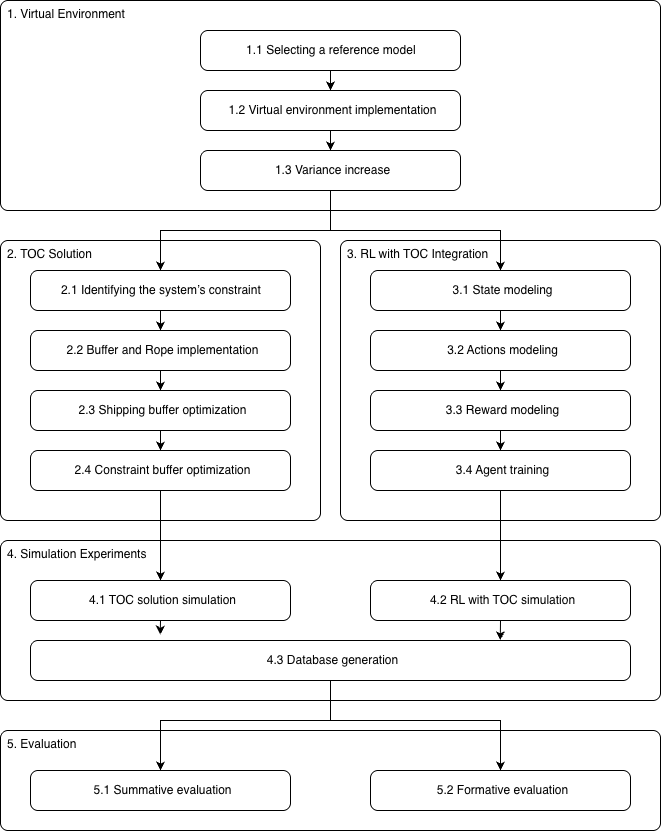
\includegraphics[width=4.08151in,height=5.13122in]{figures/fig01.png}

\protect\phantomsection\label{_Ref187516847}{}\colorbox{yellow!40}{Figure 1.}
\colorbox{yellow!40}{Overview of the research design.}

In stage 1, the virtual environment was constructed as the foundation
for creating the two subsequent simulation models in stages 2 and 3. The
process began with selecting a reference model in step 1.1. The
discrete-event simulation model proposed by (Atwater and Chakravorty,
2002a) was chosen for its ability to simulate a stochastic manufacturing
environment with multiple products, resources, and production routes
(see \colorbox{yellow!40}{\hyperref[_Ref187516873]{Figure 2}}). In step 1.2, we used this
reference model to implement the virtual environment computationally,
employing Python along with the SimPy framework for discrete-event
simulation (\colorbox{yellow!40}{Reference}) and OpenAI Gym, a toolkit for developing and
comparing RL algorithms (\colorbox{yellow!40}{Reference}). Finally, in step 1.3, we
introduced additional probabilistic elements to the validated model to
increase the variance of the virtual environment (\colorbox{yellow!40}{cf., Machado et
al., 2023}). These elements included resource changeovers and downtime,
such as time between failures and time to repair.

In stage 2, the virtual environment was used to develop a simulation
model that incorporated a TOC-based scheduling solution, combining DBR
and BM. First, an operational assessment of the virtual environment was
conducted, which led to identifying the system's constraint in step 2.1.
In step 2.2, once the constraint (i.e., the drum) was defined, the
remaining two elements of DBR --- the buffer and the rope --- were
implemented following (Schragenheim, 2010c). Two types of buffers were
considered (see \colorbox{yellow!40}{\hyperref[_Ref187516903]{Figure 3}}): (i) the CB and
(ii) the SB. The rope was implemented as a logic for creating,
scheduling, and releasing orders and raw materials at the system's
entrance, based on the consumption of both buffers. A BM policy was then
introduced and applied to optimize the reference levels of the shipping
buffers in steps 2.3 (Schragenheim, 2010c). In step 2.4, an experiment
was conducted to identify the best reference level for CB.

As in stage 2, the virtual environment informed the development of the
simulation model that integrated RL and TOC into a production scheduling
solution in stage 3. In step 3.1, fifty-two state variables were
considered, capturing the current quantity of each product being
processed throughout the system, including in the CB and SB. With
respect to the agent's actions, in step 3.2 we the decisions as how much
of each product to produce during the replenishment interval. The
scheduling and release of orders followed the logic established by TOC
(see \colorbox{yellow!40}{\hyperref[_Ref187516938]{Figure 5}}). In step 3.3, the reward
function was modeled by incorporating four penalty subfunctions aligned
with TOC's two key performance measures: (i) throughput and (ii)
inventory. Finally, in step 3.4, the PPO algorithm was employed to train
the agent in its search for the optimal policy (\colorbox{yellow!40}{cf. Reference}).
This training process was carried out across 100,000 interactions and
implemented using the Stable Baselines3 library (\colorbox{yellow!40}{Raffin et al.,
2021}).

In stage 4, both simulation models --- one based on TOC (step 4.1) and
the other integrating RL with TOC (step 4.2) --- were executed over
multiple replications (or episodes), simulating 200.000 time units of
operation. The performance measures used as model outputs included: (i)
the number of products produced and sold; (ii) the average number of
parts in process; (iii) the average lead-time; and (iv) the average
inventory, all measured over a predefined replenishment interval. In
step 4.3, these measures were recorded both by individual product and in
aggregate, resulting in a database generated from the simulation runs.

In the final stage, the database of simulation runs underwent both
summative and formative evaluations (\colorbox{yellow!40}{cf., Venable, 2016}). The
summative evaluation (step 5.1) aimed to quantify the performance
difference between the two simulation models, using the TOC-based model
as a reference. This analysis employed a confidence interval for the
paired mean difference (\colorbox{yellow!40}{cf., Law, 2015 p. 560}). The formative
evaluation (step 5.2) focused on understanding and explaining the
underlying reasons for the observed performance differences. This
process unfolded in two phases. First, three analytical techniques were
applied --- Spearman's coefficient (\colorbox{yellow!40}{Yu et al., 2021}), multiple
linear regression (\colorbox{yellow!40}{Nathans et al., 2012}), and decision trees
(\colorbox{yellow!40}{Kuhnle et al., 2022}) --- to explore the relationship between state
variables and the actions taken in each model. Based on the insights
drawn from these analyses, mechanism-based explanations were formulated
to articulate the dynamic hypotheses underlying the key differences
(\colorbox{yellow!40}{cf., Gauss et al. 2024a}). This also highlighted opportunities for
improving traditional DBR. Finally, in step 4.3, a new TOC-based
simulation model incorporating the modified DBR approach was built and
again compared with the model integrating RL and TOC. Further details
about the virtual environment and simulation models are provided in
section 4, while sections 5 and 6 present the simulation runs and the
summative and formative evaluations, respectively.

\section{Simulation Models}\label{simulation-models}

\subsection{\texorpdfstring{Virtual Environment
}{Virtual Environment }}\label{virtual-environment}

The reference model by Atwater and Chakravorty (\colorbox{yellow!40}{2002}), which serves
as the basis for constructing the virtual environment, represents a
job-shop manufacturing system that operates 24 hour per day, seven days
a week, producing ten different products. The demand and production
routes for these products are outlined in
\colorbox{yellow!40}{\hyperref[_Ref187516873]{Figure 2}} and detailed in Table S1 of the
supplementary material. Each product requires \colorbox{yellow!40}{one} unit of raw
material for production. The system utilizes 13 resources, with infinite
queue in front of each one, and cycle times that vary depending on the
specific product being produced; these cycle times are recorded in Table
S2. The reference model assumes no changeovers or downtime for the
resources. Therefore, considering
\(\mathbb{E}\left\lbrack \mathcal{T}_{j}^{CT} \right\rbrack = 0\),
\(\mathbb{E}\left\lbrack \mathcal{E}_{\forall j} \right\rbrack = 1\)\hspace{0pt}\hspace{0pt},
and the average demands from Table S1 (denoted as \(m_{i}\)), the
primary constraint in the system is resource nine, as determined by
Equation 9 (\colorbox{yellow!40}{cf., Reference}).

The virtual environment was implemented computationally using Python
3.11, with one time step representing one hour. Due to its stochastic
nature, the SimPy framework for discrete-event simulation (Eriksson
\emph{et al.}, 2022) was employed. Additionally, OpenAI Gym was used to
facilitate its subsequent integration with RL algorithms (Brockman
\emph{et al.}, 2016; Lang \emph{et al.}, 2021). The reference model
consists of a terminal system than rans for 200,000 hour (Atwater and
Chakravorty, 2002b).

To increase the variance of the virtual environment, we introduced
changeovers and downtime to the resources. The changeover time
\(\left( \mathcal{T}_{j}^{CT} \right)\) was modeled using a Normal
distribution, as this is typically applied when the operation consists
of a series of independent and sequential tasks (Yu and Ram, 2006). The
average changeover time was randomly assigned for each resource using a
Uniform distribution, \(U(0.0,\ 0.5)\). Similarly, the standard
deviation of the changeover time was defined using a Uniform
distribution, \(U(0.0,\ 0.3)\). Regarding downtime, it was applied to
all resources through distributions for the time between failures and
time to repair. Time between failures
\(\left( \mathcal{T}_{j}^{TBF} \right)\) was modeled using an
Exponential distribution, assuming that all resources are in the
maturity phase of their life cycle and thus exhibit a constant failure
rate (Sellitto and Brusius, 2017). The failure rate was randomly defined
using a Uniform distribution, \(U(0.001,\ 0.04)\). For time to repair
\(\left( \mathcal{T}_{j}^{TTR} \right)\), similar to changeover time,
the distribution was modeled using a Normal distribution, with the mean
and standard deviation defined by the Uniform distributions
\(U(5.0,\ 15.0)\) and \(U(1.0,\ 3.0)\), respectively.
\colorbox{yellow!40}{}\hyperref[_Ref187517135]{Table 1} summarizes the values used for
each resource.

{\def\LTcaptype{none} % do not increment counter
\begin{longtable}[]{@{}
  >{\raggedright\arraybackslash}p{(\linewidth - 18\tabcolsep) * \real{0.0957}}
  >{\raggedright\arraybackslash}p{(\linewidth - 18\tabcolsep) * \real{0.1204}}
  >{\raggedright\arraybackslash}p{(\linewidth - 18\tabcolsep) * \real{0.0635}}
  >{\raggedright\arraybackslash}p{(\linewidth - 18\tabcolsep) * \real{0.0914}}
  >{\raggedright\arraybackslash}p{(\linewidth - 18\tabcolsep) * \real{0.1204}}
  >{\raggedright\arraybackslash}p{(\linewidth - 18\tabcolsep) * \real{0.1149}}
  >{\raggedright\arraybackslash}p{(\linewidth - 18\tabcolsep) * \real{0.1204}}
  >{\raggedright\arraybackslash}p{(\linewidth - 18\tabcolsep) * \real{0.0635}}
  >{\raggedright\arraybackslash}p{(\linewidth - 18\tabcolsep) * \real{0.0914}}
  >{\raggedright\arraybackslash}p{(\linewidth - 18\tabcolsep) * \real{0.1065}}@{}}
\toprule\noalign{}
\multicolumn{10}{@{}>{\raggedright\arraybackslash}p{(\linewidth - 18\tabcolsep) * \real{0.9882} + 18\tabcolsep}@{}}{%
\begin{minipage}[b]{\linewidth}\raggedright
\protect\phantomsection\label{_Ref187517135}{}Table 1. Elements of
variance introduced into the virtual environment.
\end{minipage}} \\
\begin{minipage}[b]{\linewidth}\raggedright
Resource
\end{minipage} &
\multicolumn{3}{>{\raggedright\arraybackslash}p{(\linewidth - 18\tabcolsep) * \real{0.2753} + 4\tabcolsep}}{%
\begin{minipage}[b]{\linewidth}\raggedright
\(\mathcal{T}_{j}^{CT}\)\textsuperscript{(1)}
\end{minipage}} &
\multicolumn{2}{>{\raggedright\arraybackslash}p{(\linewidth - 18\tabcolsep) * \real{0.2353} + 2\tabcolsep}}{%
\begin{minipage}[b]{\linewidth}\raggedright
\(\mathcal{T}_{j}^{TBF}\)\textsuperscript{(1)}
\end{minipage}} &
\multicolumn{3}{>{\raggedright\arraybackslash}p{(\linewidth - 18\tabcolsep) * \real{0.2753} + 4\tabcolsep}}{%
\begin{minipage}[b]{\linewidth}\raggedright
\(\mathcal{T}_{j}^{TTR}\)\textsuperscript{(1)}
\end{minipage}} &
\multirow{2}{=}{\begin{minipage}[b]{\linewidth}\raggedright
\(\mathbb{E}\left\lbrack \mathcal{E}_{j} \right\rbrack\)\textsuperscript{(2,3)}
\end{minipage}} \\
\begin{minipage}[b]{\linewidth}\raggedright
\[j\]
\end{minipage} & \begin{minipage}[b]{\linewidth}\raggedright
Distribution
\end{minipage} & \begin{minipage}[b]{\linewidth}\raggedright
Mean
\end{minipage} & \begin{minipage}[b]{\linewidth}\raggedright
Std. dev.
\end{minipage} & \begin{minipage}[b]{\linewidth}\raggedright
Distribution
\end{minipage} & \begin{minipage}[b]{\linewidth}\raggedright
Failure rate
\end{minipage} & \begin{minipage}[b]{\linewidth}\raggedright
Distribution
\end{minipage} & \begin{minipage}[b]{\linewidth}\raggedright
Mean
\end{minipage} & \begin{minipage}[b]{\linewidth}\raggedright
Std. dev.
\end{minipage} \\
\midrule\noalign{}
\endhead
\bottomrule\noalign{}
\endlastfoot
1 & Normal & 0.25 & 0.09 & Exponential & 0.0098 & Normal & 5.24 & 2.97 &
0.89 \\
2 & Normal & 0.04 & 0.05 & Exponential & 0.0058 & Normal & 5.95 & 1.94 &
0.93 \\
3 & Normal & 0.42 & 0.17 & Exponential & 0.0116 & Normal & 5.28 & 1.91 &
0.86 \\
4 & Normal & 0.41 & 0.22 & Exponential & 0.0162 & Normal & 2.35 & 1.16 &
0.88 \\
5 & Normal & 0.34 & 0.10 & Exponential & 0.0252 & Normal & 6.00 & 2.16 &
0.88 \\
6 & Normal & 0.49 & 0.13 & Exponential & 0.0376 & Normal & 5.14 & 2.22 &
0.83 \\
7 & Normal & 0.16 & 0.09 & Exponential & 0.0079 & Normal & 5.31 & 1.95 &
0.92 \\
8 & Normal & 0.27 & 0.21 & Exponential & 0.0104 & Normal & 4.45 & 1.93 &
0.90 \\
9 & Normal & 0.45 & 0.23 & Exponential & 0.0045 & Normal & 2.69 & 1.21 &
0.95 \\
10 & Normal & 0.49 & 0.12 & Exponential & 0.0188 & Normal & 5.01 & 2.85
& 0.82 \\
11 & Normal & 0.39 & 0.17 & Exponential & 0.0301 & Normal & 3.15 & 2.39
& 0.85 \\
12 & Normal & 0.25 & 0.05 & Exponential & 0.0194 & Normal & 5.59 & 1.50
& 0.87 \\
13 & Normal & 0.28 & 0.07 & Exponential & 0.0171 & Normal & 2.95 & 1.71
& 0.89 \\
\multicolumn{10}{@{}>{\raggedright\arraybackslash}p{(\linewidth - 18\tabcolsep) * \real{0.9882} + 18\tabcolsep}@{}}{%
(1) Unit of time: hour; (2) Unit of Effectiveness: percentage; (3)
\(\mathbb{E}\left\lbrack \mathcal{E}_{j} \right\rbrack = \frac{\mathbb{E}\left\lbrack \mathcal{T}_{j}^{TBF} \right\rbrack}{\left( \mathbb{E}\left\lbrack \mathcal{T}_{j}^{TBF} \right\rbrack\mathbb{+ E}\left\lbrack \mathcal{T}_{j}^{TTR} \right\rbrack \right)}\).} \\
\end{longtable}
}

\subsection{TOC-Based Simulation
Model}\label{toc-based-simulation-model}

The first step in developing the TOC-based simulation model was to
identify the constraint, or the drum of the DBR (\colorbox{yellow!40}{cf., Reference}).
Using the data from \colorbox{yellow!40}{}\hyperref[_Ref187517135]{Table 1}, along with
Tables S1 and S2 in the supplementary material, and assuming
\(p = \mathrm{\Delta}\varphi = 168\) hours, it was confirmed that
resource nine was the system's constraint, as it had the highest load
(i.e., \(l_{9} = 0.99\)), according to Equation 9. Consequently, the
positions of the CB and SB was set, as outlined in
\colorbox{yellow!40}{\hyperref[_Ref187516873]{Figure 2}}.

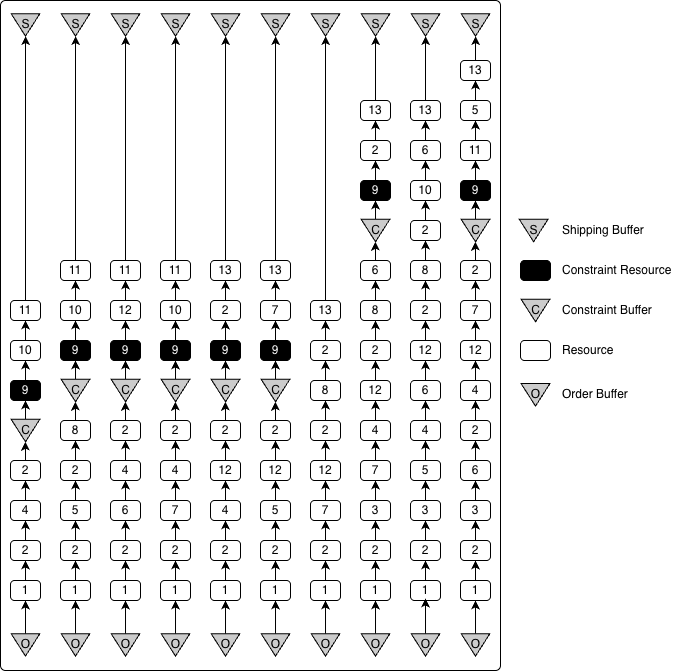
\includegraphics[width=4.64097in,height=4.53913in]{figures/fig02.png}

\protect\phantomsection\label{_Ref187516873}{}\colorbox{yellow!40}{Figure 2. Outline of
the reference model by Atwater and Chakravorty (2002).}

The implementation of the DBR rope considered three aspects, as
illustrated in \colorbox{yellow!40}{\hyperref[_Ref187516903]{Figure 3}}: (i) order
creation; (ii) scheduling; and (iii) order release. Order creation takes
place at the start of the order planning interval
\(\mathrm{\Delta}\varphi\), which in this case is \colorbox{yellow!40}{168 hours}. The
order size \(\left( M_{i}^{\mathrm{\Delta}\varphi} \right)\) is
calculated by Equation 17 and determines the reference level of the OB
for the order planning interval, i.e.,
\(\mathcal{b'}_{i}^{OB} = M_{i}^{\mathrm{\Delta}\varphi}\). Order
scheduling is modeled by Equation 15, which considers the throughput
\(\tau_{i}\) and the priority level of finished products in the SB
\(\left( \frac{\mathcal{b'}_{i}^{SB}}{H_{i}^{SB}} \right)\) (\colorbox{yellow!40}{cf.,
Reference}). In this context, we assume
\(\left( \rho_{i} - c_{i} \right) = 1\) when defining \(\tau_{i}\) in
the Equation 10, as the original work by Atwater and Chakravorty
(\colorbox{yellow!40}{2002}) does not consider the revenue and variable cost of each
product. Finally, order release, represented by
\(M_{i}^{\mathrm{\Delta}t}\), considers the consumption of the CB
\(\left( \mathcal{b'}_{i}^{CB} - H_{i}^{CB} \right)\) and the
work-in-process at each resource up to the constraint \(W_{i}^{CB}\)
(\colorbox{yellow!40}{cf., Reference}), as defined in Equation 19. The number of orders
released moderates the current level of the OB, denoted as
\(H_{i}^{OB}\).

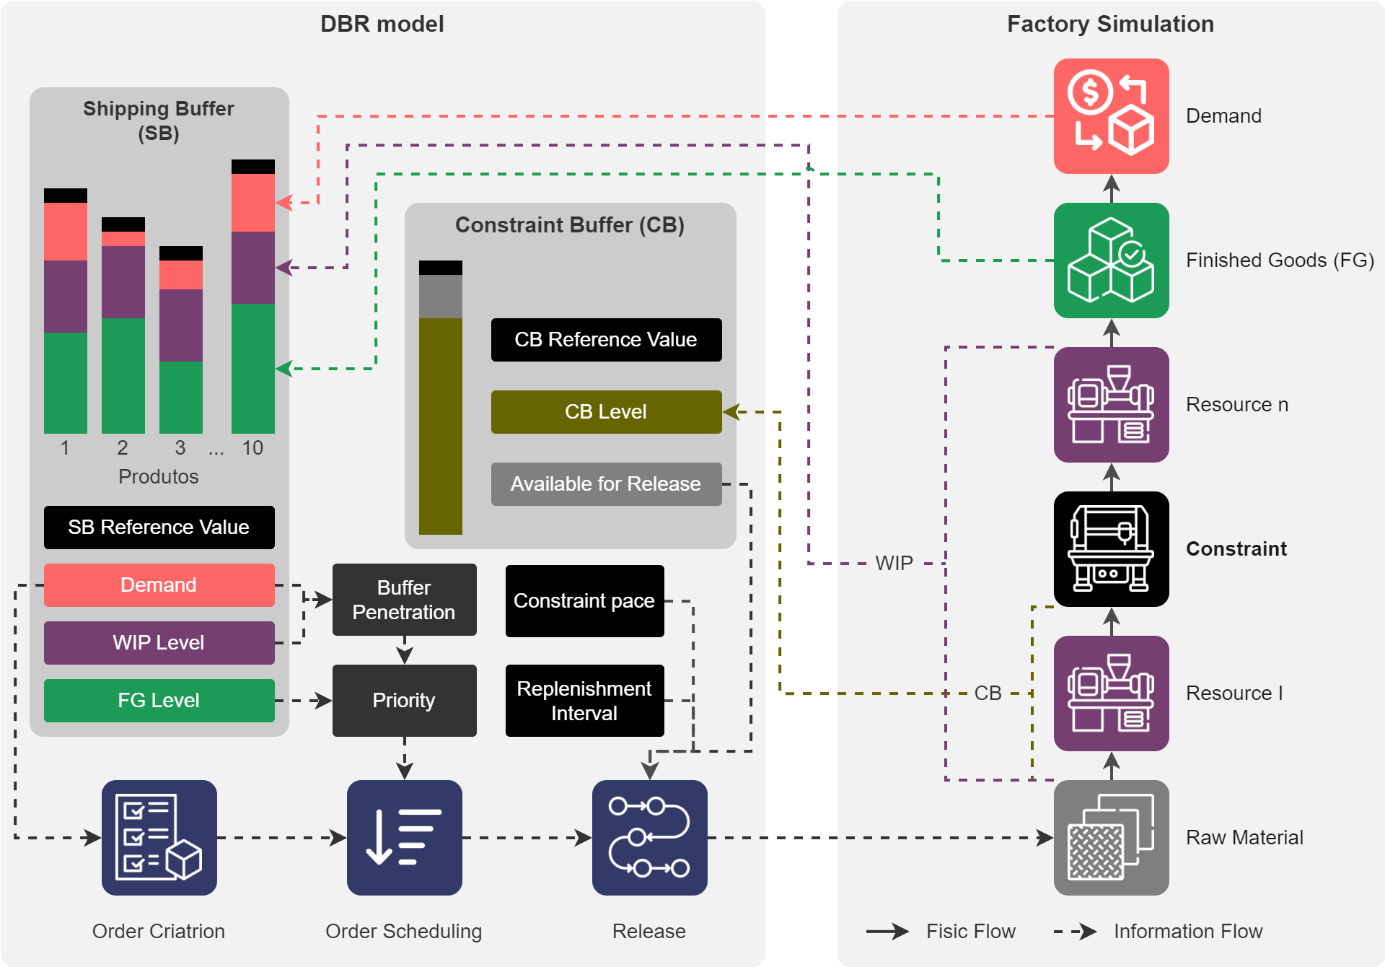
\includegraphics[width=6.29514in,height=4.39341in,alt={Diagrama Descrição gerada automaticamente}]{figures/fig03.png}

\protect\phantomsection\label{_Ref187516903}{}\colorbox{yellow!40}{Figure 3. Outline of
the TOC-based simulation model.}

The reference levels of the shipping buffers (SB) were calibrated with
the buffer-management (BM) policy described in Section 2.2. Fifteen
independent replications were run, each for 5,000,000 time units,
starting from a common oversized SB target. BM adjustments were held off
for the first 100,000 time units and then applied. For each product, the
SB target was aligned on a common time grid and averaged across
replications (Figure 4). The replication-average trajectories were
inspected graphically to identify the onset of steady state (Law, 2015).
From time 2,000,000 onward, the mean target of each replication was
computed and then averaged over the 15 replications; those values, after
rounding, were used as the fixed SB reference levels in the subsequent
experiments.

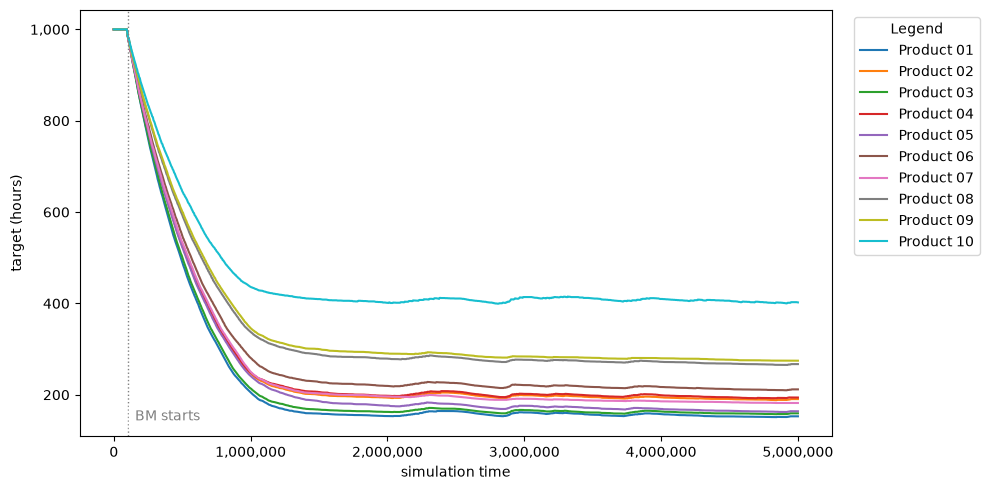
\includegraphics[width=6.29514in,height=3.12222in]{figures/fig04.png}

\colorbox{yellow!40}{Figure 4. Optimization of shipping buffer (SB) reference levels.}

The final reference level for each product in each buffer
\(\left( \mathcal{b'}_{i}^{x} \right)\), measured in terms of quantity
of semi-finished or finished products, is presented in
\hyperref[_Ref187517181]{Table 2}. These reference levels remained
constant throughout the experiments conducted in Section 5.

Table 2. Final reference leves for the shipping buffer (SB)

{\def\LTcaptype{none} % do not increment counter
\begin{longtable}[]{@{}
  >{\raggedright\arraybackslash}p{(\linewidth - 2\tabcolsep) * \real{0.3012}}
  >{\raggedright\arraybackslash}p{(\linewidth - 2\tabcolsep) * \real{0.1806}}@{}}
\toprule\noalign{}
\begin{minipage}[b]{\linewidth}\raggedright
Product \(i\)
\end{minipage} & \begin{minipage}[b]{\linewidth}\raggedright
\[\mathcal{b'}_{i}^{SB}\]
\end{minipage} \\
\midrule\noalign{}
\endhead
\bottomrule\noalign{}
\endlastfoot
1 & \colorbox{yellow!40}{0} \\
2 & \colorbox{yellow!40}{0} \\
3 & \colorbox{yellow!40}{0} \\
4 & \colorbox{yellow!40}{0} \\
5 & \colorbox{yellow!40}{0} \\
6 & \colorbox{yellow!40}{0} \\
7 & \colorbox{yellow!40}{0} \\
8 & \colorbox{yellow!40}{0} \\
9 & \colorbox{yellow!40}{0} \\
10 & \colorbox{yellow!40}{0} \\
\end{longtable}
}

The constraint-buffer (CB) target level was defined from an experiment
with 12 levels (from 250 to 800 units, in 50-unit steps), each simulated
for 50 replications. The decision used metrics with adequate sample size
(95\% CI relative half-width ≤ 5\%) that also varied significantly with
CB size (Kruskal-Wallis, α = 0.05). The level 350 was selected because
it sustained the same throughput as larger buffers while requiring the
smallest inventory, as presented on table 3.

\protect\phantomsection\label{_Ref187517181}{}Table 3. Metrics
comparison between constraint buffer (CB) target level.

{\def\LTcaptype{none} % do not increment counter
\begin{longtable}[]{@{}
  >{\raggedright\arraybackslash}p{(\linewidth - 4\tabcolsep) * \real{0.3015}}
  >{\raggedright\arraybackslash}p{(\linewidth - 4\tabcolsep) * \real{0.1686}}
  >{\raggedright\arraybackslash}p{(\linewidth - 4\tabcolsep) * \real{0.1808}}@{}}
\toprule\noalign{}
\begin{minipage}[b]{\linewidth}\raggedright
\[\mathcal{b'}_{i}^{CB}\]
\end{minipage} & \begin{minipage}[b]{\linewidth}\raggedright
\[\tau\]
\end{minipage} & \begin{minipage}[b]{\linewidth}\raggedright
\[i\]
\end{minipage} \\
\midrule\noalign{}
\endhead
\bottomrule\noalign{}
\endlastfoot
250 & \colorbox{yellow!40}{97,861} & \colorbox{yellow!40}{1,993} \\
300 & \colorbox{yellow!40}{99,884} & \colorbox{yellow!40}{2,082} \\
350 & \colorbox{yellow!40}{100,032} & \colorbox{yellow!40}{2,100} \\
400 & \colorbox{yellow!40}{100,036} & \colorbox{yellow!40}{2,105} \\
450 & \colorbox{yellow!40}{100,032} & \colorbox{yellow!40}{2,106} \\
500 & \colorbox{yellow!40}{100,036} & \colorbox{yellow!40}{2,108} \\
550 & \colorbox{yellow!40}{100,036} & \colorbox{yellow!40}{2,107} \\
600 & \colorbox{yellow!40}{100,037} & \colorbox{yellow!40}{2,109} \\
650 & \colorbox{yellow!40}{100,037} & \colorbox{yellow!40}{2,109} \\
700 & \colorbox{yellow!40}{100,036} & \colorbox{yellow!40}{2,109} \\
750 & \colorbox{yellow!40}{100,037} & \colorbox{yellow!40}{2,110} \\
800 & \colorbox{yellow!40}{100,037} & \colorbox{yellow!40}{2,110} \\
\end{longtable}
}

\subsection{RL \& TOC-Based Simulation Model {[}REVISED DRAFT -- pending
author
review{]}}\label{rl-toc-based-simulation-model-revised-draft-pending-author-review}

\noindent\colorbox{yellow!40}{REVISED DRAFT --- pending author review. Kept alongside the original version of this section below; the two have not yet been reconciled (see the reviewer note at the end of this block).}\par\medskip

The TOC \& RL-based simulation model was also built upon the virtual
environment established in Section 4.1. The state space 𝒮 comprises 22
variables: two constraint-buffer variables --- the portion of
constraint-buffer time not yet arrived at the CCR, H\^{}CB\_wip,t, and
the portion already queued at the CCR, H\^{}CB\_queue,t --- together
with, for each product i, its work-in-process level, W\_i,t, and its
finished-goods (shipping-buffer) level, H\^{}SB\_i,t:

\emph{𝒮 = \{ H\^{}CB\_wip,t , H\^{}CB\_queue,t \} ∪ \{ W\_i,t ,
H\^{}SB\_i,t \textbar{} i = 1, \ldots, I \}, I = 10}

H\^{}CB\_wip,t and H\^{}CB\_queue,t are measured in hours of processing
time still owed to the CCR and take non-negative real values; W\_i,t and
H\^{}SB\_i,t are non-negative integers. Before reaching the policy
network, all state variables are normalized online using running mean
and variance statistics accumulated during training.

This state informs the agent, which independently selects, for each
product i, the number of units to release during the replenishment
interval, forming the action space:

\emph{𝒜(𝒮) = \{ M\_i,t \textbar{} m = 0, 1, \ldots, 60 \}, i = 1,
\ldots, I = 10}

This decision is made autonomously and is not explicitly modeled by
Equation 17. Because the I = 10 products are chosen independently and
simultaneously, 𝒜(𝒮) is a multi-discrete space with 10 sub-actions of 61
categories each --- 610 discrete outputs in the policy's action layer.
The upper bound M\_i,t = 60 units was set based on the highest order
size observed in the TOC-based model over {[}xx{]} replications
{[}confirm the scaling factor applied{]}. The production sequence
follows Equation 15, and, as in the TOC-based model, it is assumed that
(ρ\_i − c\_i) = 1 when defining τ\_i in Equation 10, since the original
work by Atwater and Chakravorty (2002) does not take into account the
revenue and variable costs of the products sold. The release of orders
follows Equation 19. These relationships are illustrated in Figure 5.

The agent receives a numerical reward R\_t+1 as a result of its action
(Sutton and Barto, 2018), composed of a fixed baseline, a throughput
term, and two penalty subfunctions:

\emph{(20) R\_t+1 = R\_0 + TH\_t+1 − P\^{}LS\_t+1 − P\^{}W\_t+1 −
P\^{}SB\_t+1}

R\_0 is a fixed baseline reward added at every step. TH\_t+1 is the
throughput term; because the original work by Atwater and Chakravorty
(2002) does not provide the information needed to compute throughput as
sold value, TH\_t+1 is set to zero during training, and its role is
absorbed entirely into the lost-sales penalty P\^{}LS\_t+1. Whenever
demand for product i exceeds its current finished-goods level
H\^{}SB\_i,t, the system immediately fails to make a sale and cannot
convert inventory into throughput (cf., Reference):

\emph{(21) P\^{}LS\_t+1 = λ\_LS · Σ(i=1..I) L\_i,t}

where L\_i,t is the number of units of product i lost to unmet demand
during interval t, and λ\_LS is a penalty weight (λ\_LS = 10 during
training).

The second measure is inventory, represented by the total quantity of
items rather than monetary values, for the same reason as throughput.
Inventory is penalized through two subfunctions, one for work-in-process
and one for finished goods, each summed across the I = 10 products:

\emph{(22) P\^{}W\_t+1 = λ\_W · Σ(i=1..I) W\_i,t}

\emph{(23) P\^{}SB\_t+1 = λ\_SB · Σ(i=1..I) H\^{}SB\_i,t}

with λ\_W = 0.002 and λ\_SB = 0.001. The constraint-buffer variables
(H\^{}CB\_wip,t, H\^{}CB\_queue,t) are part of the state 𝒮 but are not
penalized directly in the reward. The overall goal is to prevent lost
sales while maintaining the lowest possible inventory level (cf.,
Schragenheim, 2010b); accordingly, λ\_SB is set lower than λ\_W.

In the RL \& TOC-based simulation model, each decision step advances the
simulation clock by the replenishment interval τ = 168 hours, matching
the order-planning interval defined for the TOC-based model in Section
4.2. An episode begins at the start of a simulation run and proceeds
through successive decision steps until either (i) the reward R\_t+1
computed for a step turns negative, ending the episode immediately (cf.
Reference), or (ii) the simulation clock reaches the 200,000-hour
horizon, truncating the episode. By incorporating the reward function
(Equation 20) into the return function (Equation 2) and assuming a
discount factor γ = 0.99, along with rewards received at future time
steps (t′ \textgreater{} t), we construct the state-value function
(Equation 3), from which the agent is trained to seek the optimal policy
π*.

The algorithm used to train the optimal policy is PPO (Schulman et al.,
2017), implemented with the Stable-Baselines3 library (Raffin et al.,
2021), using a multi-input policy network with two hidden layers of 128
units each, shared between the actor and critic branches, that
approximates both the policy and the state-value function (Russell and
Norvig, 2010; Schulman et al., 2017). Observations and rewards were
normalized online (zero mean, unit variance, clipped at ±10,000)
throughout training. Training used 8 parallel environment instances, a
rollout length of 4,096 steps per environment, mini-batches of 2,048
transitions, and 5 optimization epochs per rollout, with a learning rate
that decayed linearly from 10⁻³ to 10⁻⁴ (Equation 7) over a maximum of
16,800,000 timesteps and 277,777 episodes, the virtual environment being
reset each time the step reward turned negative (cf. Reference). The
maximum number of episodes was set based on {[}define the reason{]}
(cf., Reference). Two criteria were used to terminate the training
process (Reference): (i) the maximum number of timesteps was reached, or
(ii) return saturation occurred, where the return remained stable over
{[}xx{]} episodes.

From a computational perspective, the training process was completed in
2 hours, utilizing 15 machines running in parallel, each with the
following specifications: an i5-13450HX processor, 16 GB of RAM, and an
NVIDIA GeForce RTX 4050 graphics card. A state-value of 0.996 was
achieved after 13,888 episodes, as shown in Figure 6a. The behavior of
the penalty subfunctions is also illustrated in Figure 6b--d.

\emph{{[}Reviewer note: Figure 6's original caption lists four
penalty-subfunction panels --- lost sales, work-in-process, CB level,
and SB level ((b)--(e)) --- but the reward above has only three: lost
sales, work-in-process, and SB/finished-goods (Equations 21--23), with
no CB term. Panel (d), the CB-level curve, should be removed, and the
current panel (e) (SB) should become the new panel (d), so the caption
reads: (a) return; (b) lost-sales penalty; (c) work-in-process penalty;
(d) finished-goods (SB) penalty. With this change, the body text's
existing ``Figure 6b--d'' citation is already correct and needs no
further edit.{]}}

\bigskip\noindent\hrulefill\par\smallskip\noindent\textbf{Original version} (kept for comparison --- the revised draft above and this original section have not yet been reconciled by the author).\par\bigskip

\subsection{RL \& TOC-Based Simulation
Model}\label{rl-toc-based-simulation-model}

The TOC \& RL-based simulation model was also built upon the virtual
environment established in Section 4.1. Fifty variables were used to
represent the state space of the environment at each time step \(t\),
i.e.,
\(\mathcal{S =}\left\{ H_{i_{t}}^{OB},H_{i_{t}}^{CB},H_{i_{t}}^{SB},W_{i_{t}}^{CB},W_{i_{t}}^{SB}\ |\ h \in \mathbb{Z,\ }w = 0,\ 1,\ \ldots,\ 13 \right\}_{i = 1}^{I = 10}\).
The true buffer levels \((h)\) can take any integer value, being
negative when demand exceeds the buffer reference level, particularly
for SB. The true values of work-in-process \((w)\) can range from 0 to
13, with 13 occurring when all resources \(j\) in the longest production
route are occupied (see \colorbox{yellow!40}{\hyperref[_Ref187516873]{Figure 2}} and
Table S1). This state space informs the agent, which selects the number
of products to produce during the replenishment interval from a set of
\colorbox{yellow!40}{210} possible actions, i.e.,
\(\mathcal{A(S) =}\left\{ M_{i_{t}}\ |\ m = 0,\ 1,\ldots,\ 20 \right\}_{i = 1}^{I = 10}\).
This decision is made autonomously and is not explicitly modeled by
Equation 17. The quantity of each product to be produced ranges from 0
to \colorbox{yellow!40}{20}, with 0 representing the decision to produce nothing. The
maximum limit of \colorbox{yellow!40}{20} was set based on the highest order size
observed in the TOC-based model after \colorbox{yellow!40}{xx} replications and then
duplicated. The production sequence follows Equation 15, but similarly
to the TOC-based model, it is assumed that
\(\left( \rho_{i} - c_{i} \right) = 1\) when defining \(\tau_{i}\) in
Equation 10, since the original work by Atwater and Chakravorty
(\colorbox{yellow!40}{2002}) does not take into account the revenue and variable costs of
the products sold. The release of orders follows Equation 19. These
relationships are illustrated in \colorbox{yellow!40}{\hyperref[_Ref187516938]{Figure
5}}.

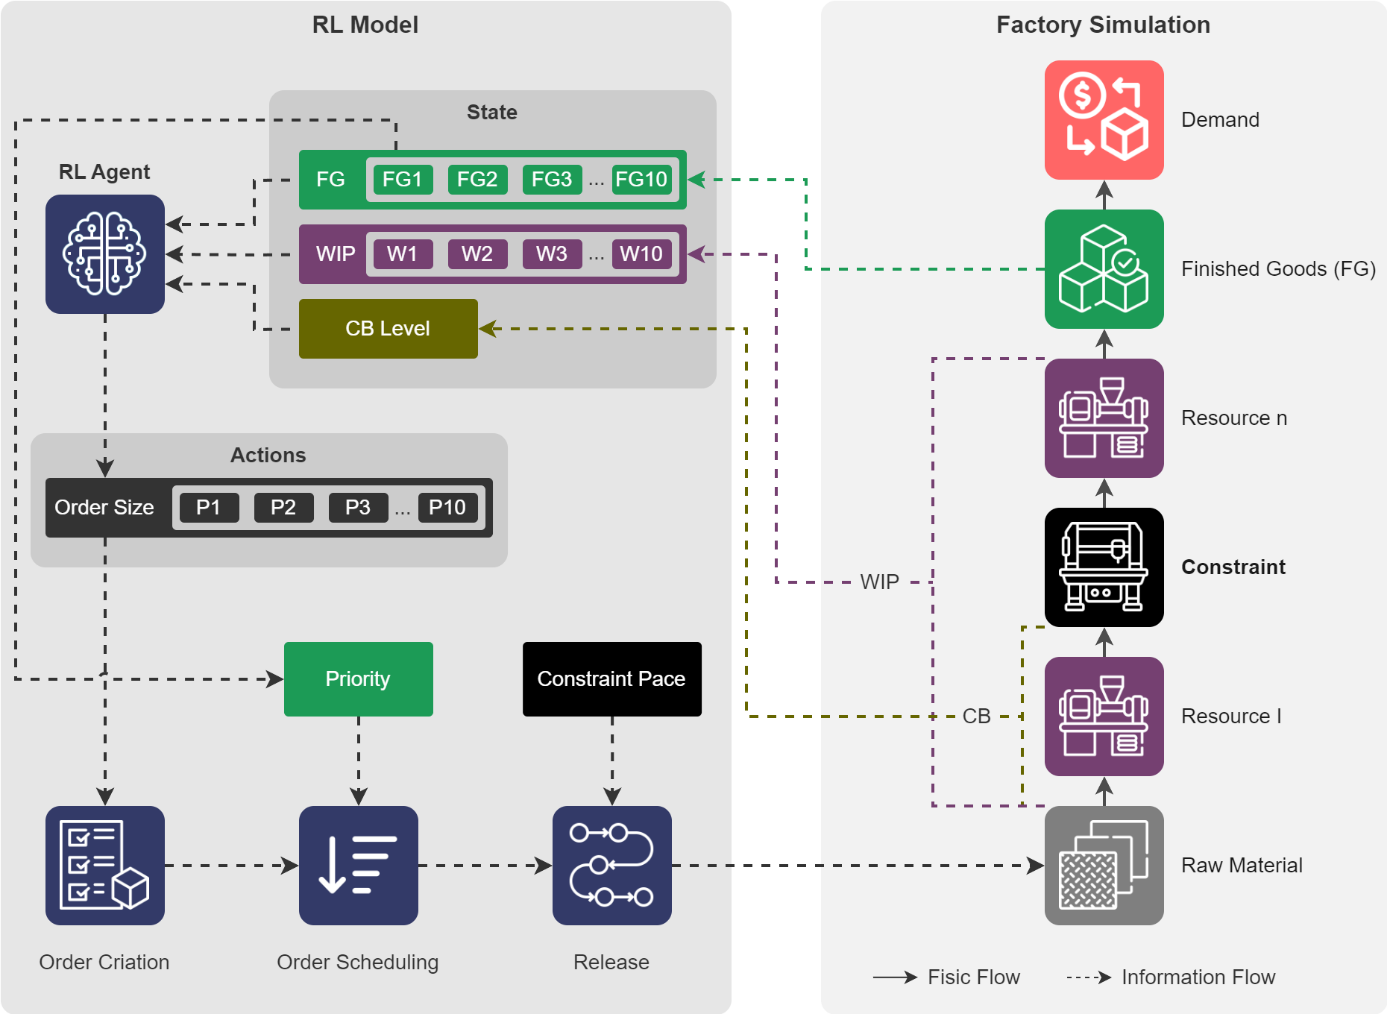
\includegraphics[width=6.29514in,height=4.60302in,alt={Diagrama Descrição gerada automaticamente}]{figures/fig05.png}

\protect\phantomsection\label{_Ref187516938}{}\colorbox{yellow!40}{Figure 5. Outline of
the RL \& TOC-based simulation model.}

The agent receives a numerical reward \(R_{t + 1}\) as a result of its
action (Sutton and Barto, 2018). Two of the performance measures from
the TOC are implicitly used as penalty subfunctions within the following
reward function:

\begin{equation}
R_{t + 1}\  = \frac{1}{I}\sum_{\forall i}^{}{1 - P_{i_{t + 1}}^{\tau} - P_{i_{t + 1}}^{W^{SB}} - P_{i_{t + 1}}^{H^{CB}} - P_{i_{t + 1}}^{H^{SB}}}.
\tag{20}
\end{equation}

The first of these measures is throughput \((\tau)\), which, due to the
original work by Atwater and Chakravorty (\colorbox{yellow!40}{2002}) lacking information
for its calculation, is treated as a penalty for lost sales (\colorbox{yellow!40}{cf.
Reference}). In other words, whenever the demand for a product exceeds
its current level in the SB, the system immediately fails to make a sale
and, consequently, cannot convert inventory into throughput (\colorbox{yellow!40}{cf.,
Reference}). This penalty is incurred whenever the SB level is negative.
Equation 21 outlines this condition, weighted by a factor of 0.3, which
gives greater importance to this penalty:

\begin{equation}
P_{i_{t + 1}}^{\tau} = \left\{ \binom{0.3H_{i_{t}}^{SB}\ }{0\ \ \ \ \ \ \ \ \ \ \ \ }\binom{if\ H_{i_{t}}^{SB} < 0}{if\ H_{i_{t}}^{SB} \geq 0} \right.\ .
\tag{21}
\end{equation}

The second measure is inventory \(\mathcal{(i)}\), which in the model is
represented by the quantity of items rather than monetary values, for
the same reason as throughput. Inventory is divided into three penalty
subfunctions, each squared, to amplify the impact of larger values
(\colorbox{yellow!40}{cf., Reference}). The first subfunction penalizes work-in-process
throughout the system, \(P_{i_{t + 1}}^{W^{SB}}\). The second penalizes
the level of the CB, \(P_{i_{t + 1}}^{H^{CB}}\), while the third
penalizes the number of items in the SB, \(P_{i_{t + 1}}^{H^{SB}}\). The
overall goal is to prevent lost sales while maintaining the lowest
possible inventory level (\colorbox{yellow!40}{cf., Schragenheim, 2010b}). For this
reason, the weight is smaller in Equation 24, while the other equations
have equal weights.

\begin{equation}
P_{i_{t + 1}}^{W^{SB}} = \left( 0.02W_{i_{t}}^{SB} \right)^{2};
\tag{22}
\end{equation}

\begin{equation}
P_{i_{t + 1}}^{H^{CB}} = \left( 0.02H_{i_{t}}^{CB} \right)^{2};
\tag{23}
\end{equation}

\begin{equation}
P_{i_{t + 1}}^{H^{SB}} = \left( 0.01H_{i_{t}}^{SB} \right)^{2};
\tag{24}
\end{equation}

In the RL \& TOC-based simulation model, the natural event that
determines the length of each simulation run, or episode in
reinforcement learning terminology (\colorbox{yellow!40}{cf., Reference}), is the
\colorbox{yellow!40}{72}-hour replenishment interval \((\mathrm{\Delta}\varphi)\). By
incorporating the reward function (Equation 21) into the return function
(Equation 2) and assuming a discount factor \(\gamma = 0.0\), along with
rewards received at future time steps (\(k = 71\)), we can construct the
state value function (Equation 3), from which the agent can be trained
to seek the optimal policy, \(\pi_{*}\).

The algorithm used for training the optimal policy is PPO (\colorbox{yellow!40}{Schulman
et al., 2017}), implemented using the Stable Baselines 3 library
(\colorbox{yellow!40}{Raffin et al., 2021}), which employs neural networks to approximate
both the policy and the state-value function (\colorbox{yellow!40}{Russell and Norvig,
2010; Schulman et al., 2017}). A learning rate of
\(\epsilon = 0.0002\ \) (Equation 7) and a maximum number of 277,777
replications (or episodes) were used during training, with the virtual
environment being reset each time the return reached zero (\colorbox{yellow!40}{cf.
Reference}). The maximum number of episodes was set based on
{[}\colorbox{yellow!40}{define the reason}{]} (\colorbox{yellow!40}{cf., Reference}). Two criteria were
used to terminate the training process (\colorbox{yellow!40}{Reference}): (i) the maximum
number of episodes was reached, or (ii) return saturation occurred,
where the return remained stable over \colorbox{yellow!40}{xx} episodes.

From a computational perspective, the training process was completed in
2 hours, utilizing 15 machines running in parallel, each with the
following specifications: an i5-13450HX processor, 16 GB of RAM, and an
NVIDIA GeForce RTX 4050 graphics card. A \colorbox{yellow!40}{state-value of 0.996} was
achieved after 13,888 episodes, as shown in
\colorbox{yellow!40}{\hyperref[_Ref187516969]{Figure 6}}a. The behavior of penalty
subfunctions is also illustrated in \colorbox{yellow!40}{\hyperref[_Ref187516969]{Figure
6}}b-d.

\begin{figure}[htbp]
\centering
\begin{subfigure}[b]{\textwidth}
\centering
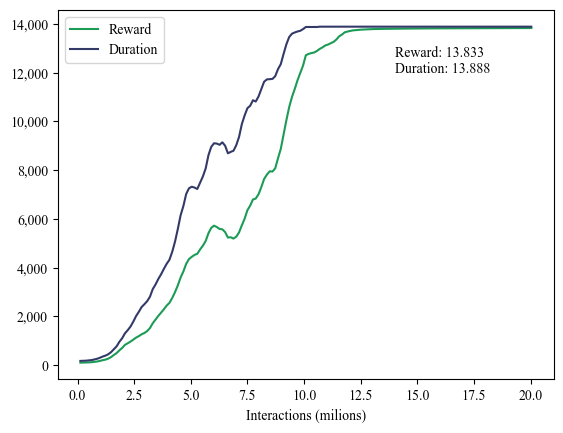
\includegraphics[width=\linewidth]{figures/fig06a.png}
\caption{}
\label{fig:sub:a}
\end{subfigure}
%
\begin{subfigure}[b]{0.48\textwidth}
\centering
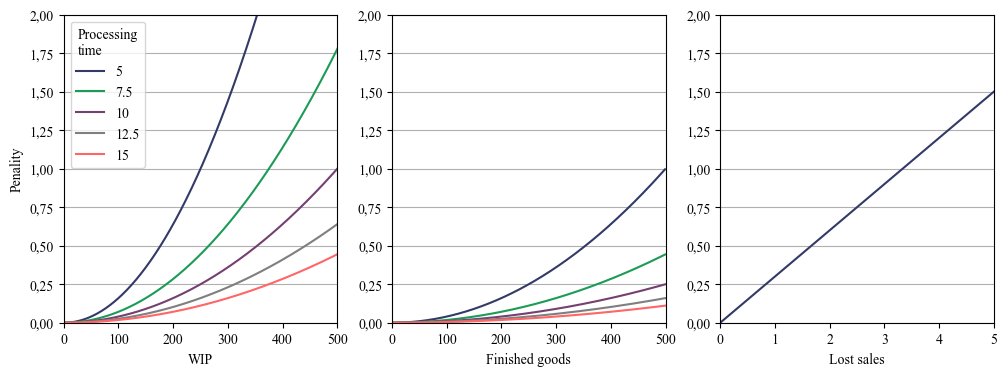
\includegraphics[width=\linewidth]{figures/fig06bcde.png}
\caption{}
\label{fig:sub:b}
\end{subfigure}
\begin{subfigure}[b]{0.48\textwidth}
\centering
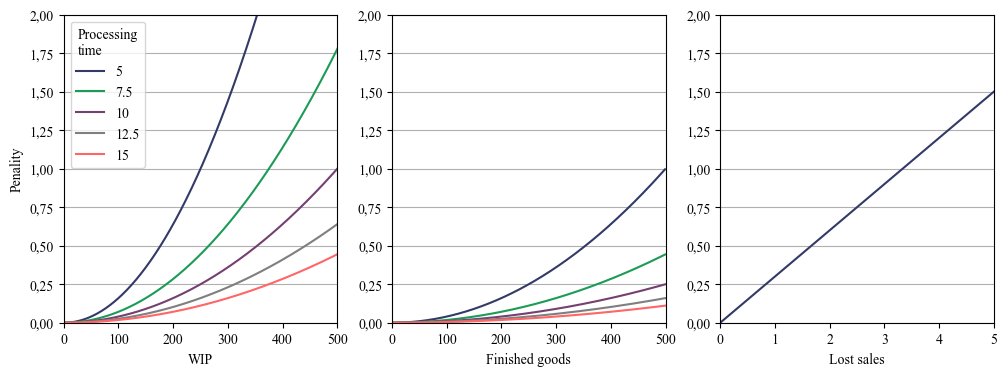
\includegraphics[width=\linewidth]{figures/fig06bcde.png}
\caption{}
\label{fig:sub:c}
\end{subfigure}
%
\begin{subfigure}[b]{0.48\textwidth}
\centering
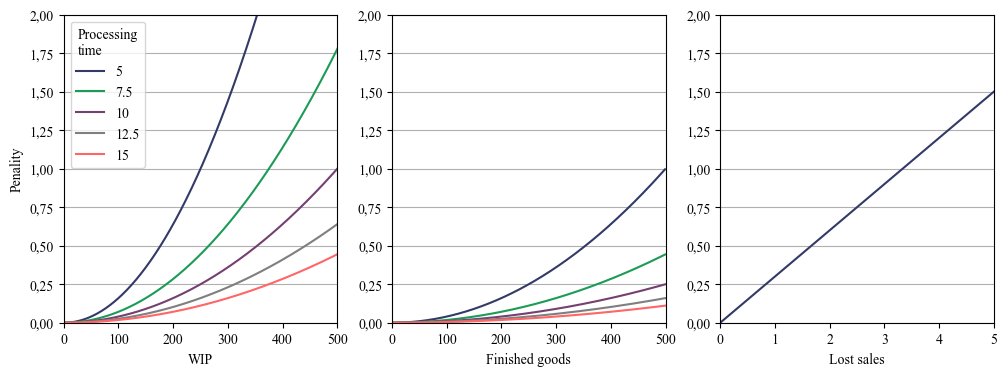
\includegraphics[width=\linewidth]{figures/fig06bcde.png}
\caption{}
\label{fig:sub:d}
\end{subfigure}
\begin{subfigure}[b]{0.48\textwidth}
\centering
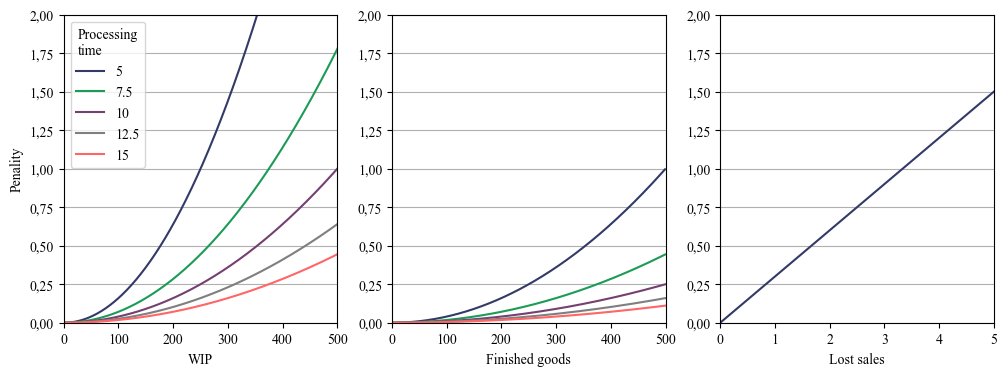
\includegraphics[width=\linewidth]{figures/fig06bcde.png}
\caption{}
\label{fig:sub:e}
\end{subfigure}
%
\caption{\protect\phantomsection\label{_Ref187516969}{}\colorbox{yellow!40}{Figure 6. Dynamic
behaviour of: (a) the return function; (b) the penalty subfunction for
lost sales; (c) the penalty subfunction for work-in-process; (d) the
penalty subfunction for the CB level; and (e) the penalty subfunction
for the SB level.}}
\end{figure}

\section{Execution of Simulation
Experiments}\label{execution-of-simulation-experiments}

The two simulation models --- one based on TOC and the other integrating
RL with TOC --- were run across 52 replications (or episodes),
representing one year of operation. Each replication simulated a 72-hour
order planning interval, corresponding to a five-day workweek with two
7.2-hour shifts per day. The performance measures used as model outputs
included: (i) the number of products produced and sold; (ii) the average
number of parts in process; (iii) the average level of the CB; and (iv)
the average level of the SB, all measured over a predefined
replenishment interval. These metrics were captured both per product and
in aggregate, generating a database from the simulation runs. Further
details can be found in Tables S4-S11 of the supplementary material.

\section{Summative and Formative
Evaluations}\label{summative-and-formative-evaluations}

The results were analyzed in two stages: (i) productivity analysis and
(ii) behavior analysis. The productivity analysis compares the
production performance of the two scheduling approaches, while the
behavior analysis explains how these results were achieved.

To compare the performance of the two scheduling methods, hypothesis
tests were conducted to determine whether there were statistically
significant differences (\colorbox{yellow!40}{\hyperref[_Ref187517011]{Figure 7}}).
Specifically, each test examined the null hypothesis that both
scheduling methods come from the same probability distribution. Because
at least one sample in each comparison failed the Shapiro--Wilk
(normality) or Levene (homoscedasticity) tests, the Wilcoxon test was
used instead of the two-sample t-test (Law, 2015; Telles \emph{et al.},
2020b). The Wilcoxon test was performed at a 95\% confidence level and a
5\% significance level (\colorbox{yellow!40}{}\hyperref[_Ref187517192]{Table 3}).

\begin{figure}[htbp]
\centering
\begin{subfigure}[b]{0.48\textwidth}
\centering
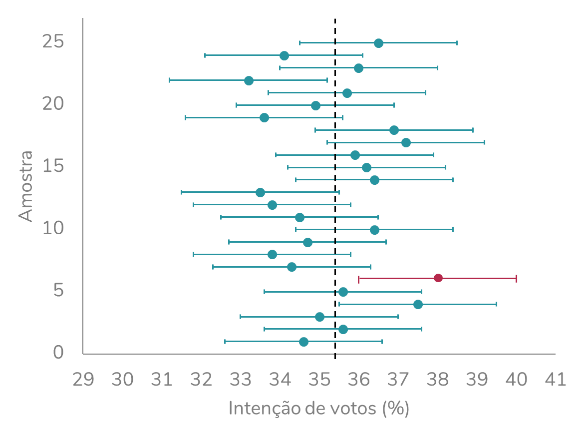
\includegraphics[width=\linewidth]{figures/fig07abcd.png}
\caption{}
\label{fig:sub:a}
\end{subfigure}
\begin{subfigure}[b]{0.48\textwidth}
\centering
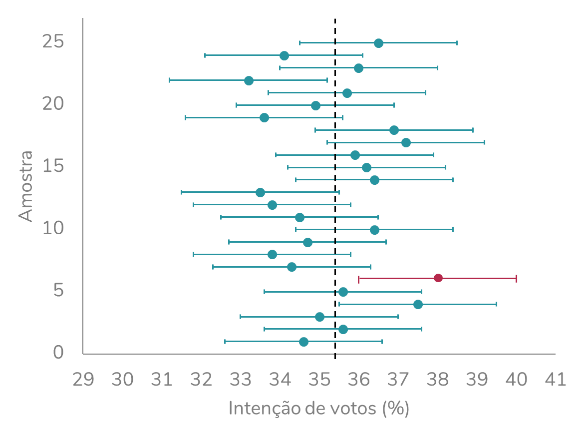
\includegraphics[width=\linewidth]{figures/fig07abcd.png}
\caption{}
\label{fig:sub:b}
\end{subfigure}
%
\begin{subfigure}[b]{0.48\textwidth}
\centering
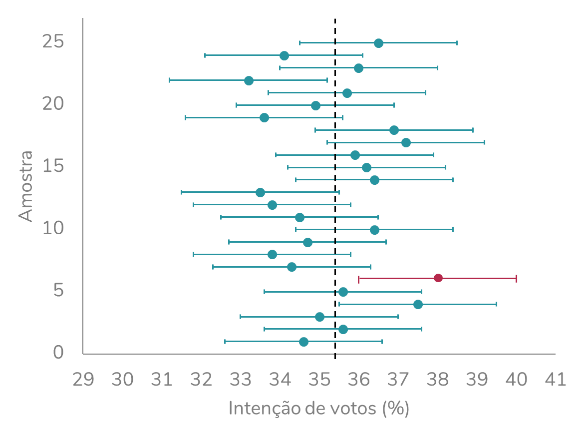
\includegraphics[width=\linewidth]{figures/fig07abcd.png}
\caption{}
\label{fig:sub:c}
\end{subfigure}
\begin{subfigure}[b]{0.48\textwidth}
\centering
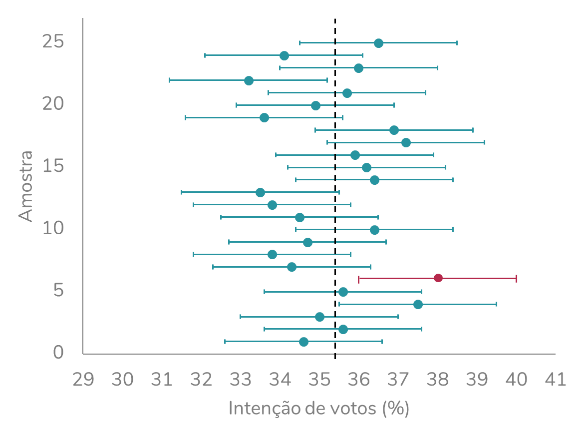
\includegraphics[width=\linewidth]{figures/fig07abcd.png}
\caption{}
\label{fig:sub:d}
\end{subfigure}
%
\caption{\protect\phantomsection\label{_Ref187517011}{}\colorbox{yellow!40}{Figure 7. Confidence
intervals of the differences for: (a) the number of products produced
and sold; (b) the average number of parts in process; (c) the average
level of the CB; and (d) the average level of the SB.}}
\end{figure}

The results indicate no statistically significant differences in demand
(DM) or quantity of products sold (SP), showing that both approaches met
demand equally. However, throughput time (FT), work in process (WIP),
finished goods (FG), and total inventory (IV) levels are lower under the
RL approach.

Behavioral analysis was conducted using three techniques to examine the
relationship between state variables and the scheduling decisions. The
first technique, Spearman's correlation, evaluates the monotonic
relationship between two quantitative variables without requiring
linearity (Barbosa and Azevedo, 2018; Xiao \emph{et al.}, 2015). The
correlation analysis shows that DBR exhibits a negative relationship
between FG and WIP for the same product, reflecting the DBR mechanism
that maintains the shipping buffer (SB) at its reference value
regardless of production stage, thus balancing FG and WIP. The FG and
WIP levels of different products behave similarly, except for products 7
and 9, which are unrestricted and released based on consumption. Actions
showed no significant correlations with state variables, apart from weak
correlations in products 2, 6, 7 (with FG), and product 9 (with WIP).
The RL agent reveals a similar pattern regarding the relationship
between FG and WIP, particularly for products 7 and 9 though the
correlation is weaker. This implies that while the RL agent also seeks
to balance FG and WIP, additional factors influence its decisions.
Unlike DBR, the RL agent exhibits weak to moderate negative correlations
between the action and the respective WIP (except for product 9). This
negative correlation suggests that the RL agent prioritizes releasing
materials when WIP is low, a behavior not observed in DBR. The results
from both correlations can be found in appendix.

The second approach used linear regression to identify the contribution
of WIP and FG on the quantity of products released by the scheduling
methods. A linear regression was run for each product, treating WIP and
FG as independent variables and the quantity of products released as the
dependent variable (full table in appendix). The result shows that the
DBR actions display a strong linear relationship with state variables,
with coefficients of determination exceeding 80\%. The primary
influencing factors are the product's own WIP and FG levels, while the
constraint buffer (CB) has no discernible impact. RL shows lower
coefficients of determination, below 55\%. Although WIP and FG remain
the key decision variables, the influence of CB is again negligible.
However, RL's decisions are less strongly determined by WIP and FG than
DBR's, indicating additional complexities in the agent's decision-making
process.

To complement the analysis and make RL decisions readable, a Decision
Tree model was trained for each action based on the RL agent's
state--action history. In DBR, WIP and FG collectively account for more
than 85\% of the decision's explanatory power. In the RL agent, WIP
exerts more influence than FG, but combined they explain less than 50\%
of the decision-making process for each action
(\colorbox{yellow!40}{}\hyperref[_Ref187517031]{Figure 8}). Unlike DBR, where other
products' variables have minimal effect, several RL actions show up to
5\% influence from variables related to other products, underscoring a
more nuanced decision process.

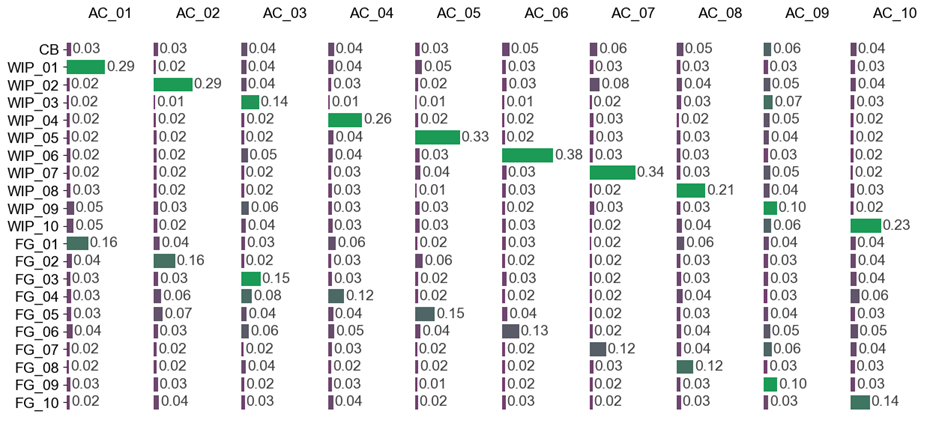
\includegraphics[width=6.30069in,height=2.9in]{figures/fig08.png}

\protect\phantomsection\label{_Ref187517031}{}Figure 8. Decision tree
influence of variables on RL actions

The number of nodes in a decision tree reflects how many rules are
required to explain the dataset (Myles \emph{et al.}, 2004; Rudin
\emph{et al.}, 2022). In this study, the DBR decision trees use fewer
nodes than their RL counterparts (\colorbox{yellow!40}{}\hyperref[_Ref187517024]{Figure
9}) indicating that the RL scheduling approach makes more complex
decisions. For DBR, products 7 and 9 exhibit the simplest trees because
they are not processed by the constraint, so their material release
depends only on the respective shipping buffer (SB). Conversely,
products 8 and 10 have the most complex trees, consistent with the fact
that they pass through the constraint and involve more processing steps.
In contrast, the RL decision trees do not show a clear pattern relating
the number of nodes to the model's dynamics. Notably, product 9 has the
largest tree in RL's case, despite not being processed by the
constraint.

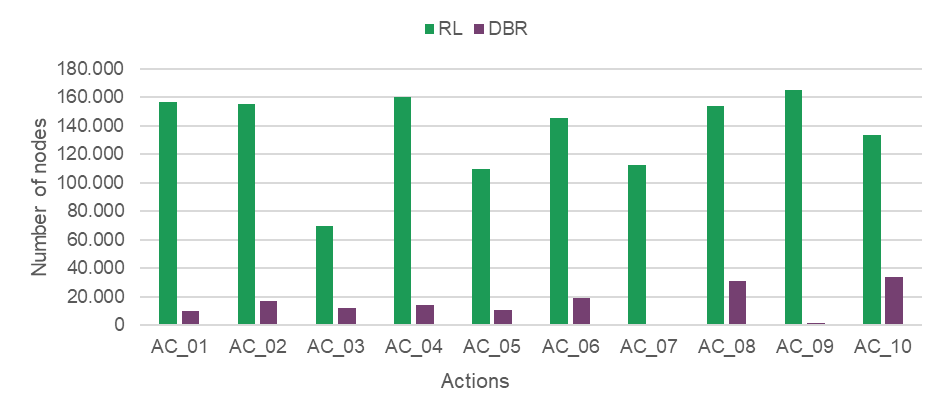
\includegraphics[width=6.30069in,height=2.76042in]{figures/fig09.png}

\protect\phantomsection\label{_Ref187517024}{}Figure 9. Quantity of
decision tree nodes.

\section{Discussion}\label{discussion}

Integrating RL with DBR reduced inventory and shortened throughput
times, thereby increasing production system efficiency by treating the
shipping buffer (SB) as both WIP and FG. From a TOC standpoint, lower
inventory boosts return on investment (ROI) and strengthens cash flow
(Gupta \emph{et al.}, 2002; Machado \emph{et al.}, 2023). It also
mitigates system variability by reducing queues at the resources
(Goldratt, 2006a; Machado \emph{et al.}, 2023). Shorter queues, in turn,
improve lead times, allowing for quicker responses to demand
fluctuations and machine breakdowns (Thürer \emph{et al.}, 2022). By
decomposing the SB into WIP and FG, this approach eliminates the need to
maintain a fixed SB reference value and continuously adjust it,
ultimately streamlining decision-making and enhancing production
efficiency.

The principles of TOC were instrumental in shaping the RL model,
particularly in defining the state and reward function. Since the state
must provide all the information for the agent to make decisions (Sutton
and Barto, 2018), incorporating the SB concept enables the RL agent to
effectively understand the system\textquotesingle s production needs and
meet demand. This approach eliminates the need for comprehensive
monitoring of the production system, such as tracking queued products
(Shiue \emph{et al.}, 2020; Thomas \emph{et al.}, 2018), order
characteristics (Liu \emph{et al.}, 2022; Marchesano \emph{et al.},
2022), or the status and utilization of resources (Liu \emph{et al.},
2022; Sakr \emph{et al.}, 2023). Furthermore, the reward function,
designed based on TOC performance metrics (gain and inventory), has
proven sufficient for training the RL algorithm and has demonstrated its
effectiveness in decision-making.

Typically, RL scheduling methods are limited to scheduling predefined
production orders (Esteso \emph{et al.}, 2023). However, integrating RL
with DBR allows the agent to determine order sizes while scheduling
production based on the volume of finished goods in stock. This approach
adapts RL to a make-to-stock (MTS) environment, contrasting with the
more common focus on make-to-order (MTO) systems (Panzer and Bender,
2022). It also increases the autonomy of the scheduling process,
aligning with the aim of autonomous decision-making in Industry 4.0 (Jan
\emph{et al.}, 2023; Oztemel and Gursev, 2020). Although DBR scheduling
performed effectively in the simulation model, its integration with RL
achieved equivalent productivity while reducing both inventory and
throughput time (\colorbox{yellow!40}{}\hyperref[_Ref187517192]{Table 3}).

Correlation analysis, linear regression, and decision trees were used to
explain the RL agent's decisions, with DBR serving as a baseline for
comparison. These methods confirmed that DBR's behavior aligns with its
underlying model, highlighting how SB levels influence product quantity
decisions (Schragenheim, 2010c). In contrast, the RL agent prioritizes
WIP more than FG when deciding what quantities to produce, showing a
result of RL's capacity to learn the system's dynamics and adapt to
disruptions such as machine breakdowns. This phenomenon is illustrated
in \hyperref[_Ref187517040]{Figure 10}. When resource III experiences a
breakdown (red bar at time T2), parts accumulate in front of the
resource while the market continues to consume the FG. As FG levels
decrease, a new order is released to restore the SB level, leading to an
increase in WIP (time T3). By times T4 and T5, the levels of WIP and FG
return to their initial values due to the protective capacity of the
resources, and product releases continue in accordance with the SB
level.

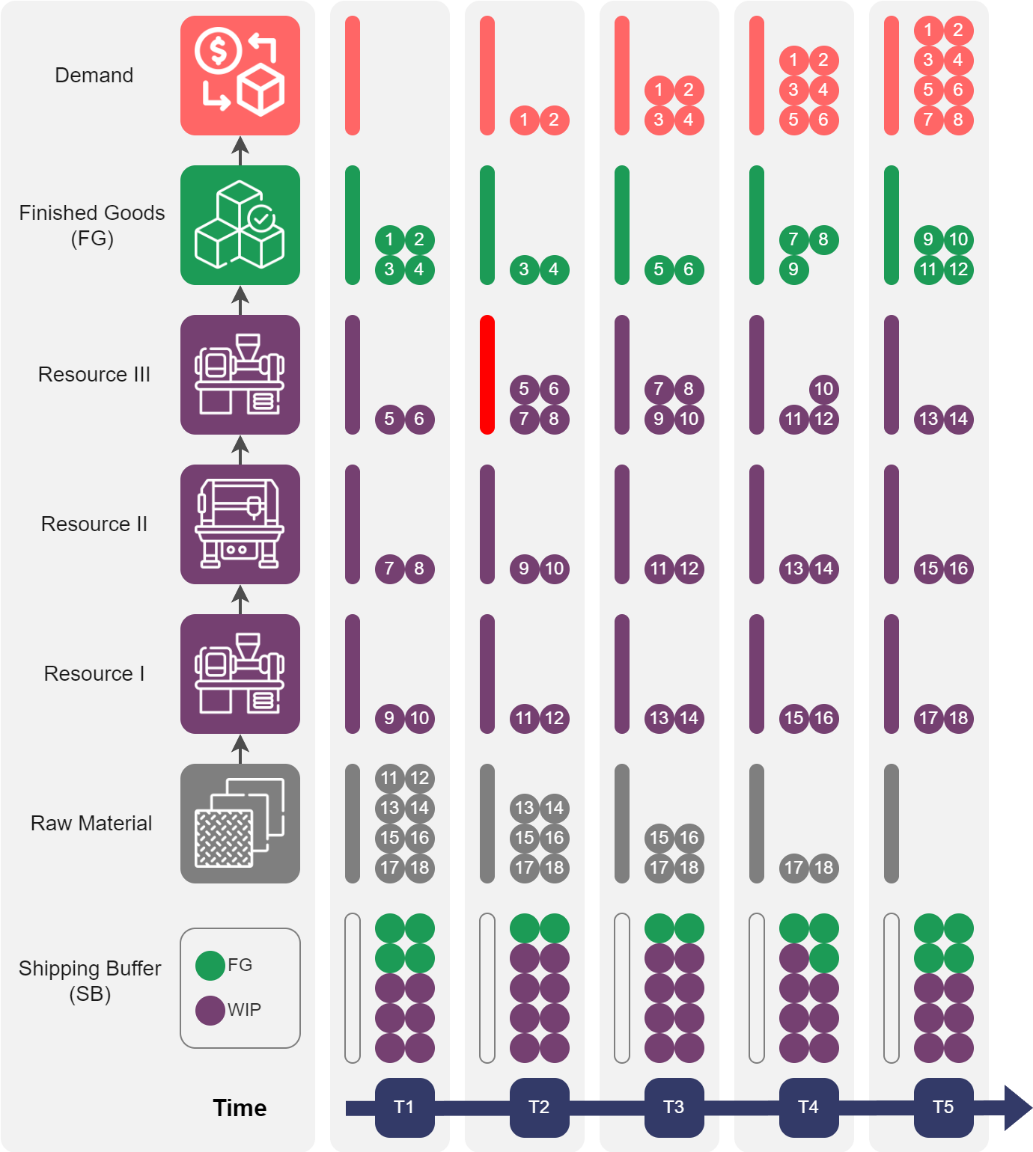
\includegraphics[width=4.68918in,height=5.23285in,alt={Diagrama Descrição gerada automaticamente com confiança baixa}]{figures/fig10.png}

\protect\phantomsection\label{_Ref187517040}{}Figure 10. Machine
breakdown in the DBR.

By highlighting RL\textquotesingle s performance, it becomes evident
that there is potential for improving DBR, particularly by considering
WIP as a standalone decision-making variable rather than treating it
solely as part of the SB. Although no direct relationship between WIP
and the number of products released was identified, the decision tree's
node count reveals a significant difference between the two scheduling
methods. This discrepancy suggests that other variables or combinations
of variables may influence decisions in certain system states. However,
defining these relationships comprehensively can be both labor-intensive
and, in some cases, infeasible (Kuhnle \emph{et al.}, 2022; Rudin
\emph{et al.}, 2022).

\section{Conclusions}\label{conclusions}

This study represents a first attempt to integrate RL with DBR for
production scheduling. The RL model was developed using TOC concepts and
trained within a DES environment modeled on DBR studies, simulating a
job shop with stochastic processes. Modifications, including machine
setups and equipment breakdowns, were introduced to evaluate the
solution's performance in scenarios with high variability. The results
showed that RL achieved the same level of productivity as DBR but with
lower inventory levels.

The primary contribution of this research lies in enhancing production
scheduling efficiency by integrating RL with TOC principles and
decomposing the SB into WIP and FG. Additionally, the analysis of RL
behavior identified WIP as the key variable influencing product release
decisions, highlighting opportunities to refine DBR by incorporating WIP
more prominently. While the exact influence of WIP on RL actions could
not be fully determined, integrating RL with DBR significantly improved
the production system by reducing inventory and shortening throughput
times. Furthermore, incorporating TOC concepts into RL modeling enabled
effective decision-making without the need for exhaustive production
monitoring.

Regarding limitations, this study's simulation model is theoretical,
incorporating simplified representations of reality that exclude
operational costs and system gains (Goldratt, 2006a). Consequently,
economic analyses, including the TOC-proposed prioritization of product
mix, were not performed. Additionally, the MTS operating mode used in
this study did not account for the potential to operate in an MTO
framework. Future research opportunities include implementing the
proposed solution in more complex environments using empirical data,
comparing the RL model with alternative approaches, and further
exploring DBR by isolating WIP and FG as individual decision-making
variables.

This study adopted a mechanism-based perspective to explore whether and
how TOC can enhance Lean production theory in the context of optimizing
a welding line in a manufacturing company. We applied Lean and TOC
principles to design and implement an intervention that increases the
economic efficiency of this line by more than 230 percent. The
intervention challenged three assumptions underlying Lean implementation
and sustainment: (i) inventory and capacity buffers are cost equivalent;
(ii) reducing variability is the primary way to synchronize production
with demand; and (iii) continuous improvement inherently leads to
efficiency improvements. It also challenges the TOC assumption that
increased demand has no limit, but reduced inventory and operating
expenses do. As such, our study sheds light on the rationale for
economic efficiency-centered design that goes beyond the Lean and TOC
lenses. This rationale is grounded in the following kinematic
mechanisms: (i) measuring production systems in terms of economic
efficiency; (ii) synchronizing production and demand by eliminating
obvious waste and reducing and/or buffering variability; and (iii)
managing progress toward the economic efficiency frontier by means of
system constraints.


\nocite{*}
\printbibliography

\end{document}
